\documentclass[10pt]{beamer}
\usetheme[progressbar=frametitle]{metropolis}
\includeonlyframes{}
%%%%%%%%%%%%%%%%%%%%%%%%%%%%%%%%%%%%%%%%%%%%%%%%%%%%%%%%%%%%%%%%%%%%%%%%%%%%%%%%
%					Preambulo
%%%%%%%%%%%%%%%%%%%%%%%%%%%%%%%%%%%%%%%%%%%%%%%%%%%%%%%%%%%%%%%%%%%%%%%%%%%%%%%%
\usepackage[spanish,activeacute]{babel}
\usepackage{xcolor}
\usepackage{color}
\usepackage{colortbl}
\usepackage{amsmath}
\usepackage{amssymb}
\usepackage{graphicx}
\usepackage{latexsym}
\usepackage{ucs}
\usepackage[utf8]{inputenc}
\usepackage{wrapfig}
\usepackage{siunitx}
\usepackage{times}
\usepackage{tikz}
\usepackage{verbatim}
\usepackage{multimedia}
\usepackage{hyperref}
\usepackage{thumbpdf}
\usepackage{wasysym}
\usepackage{pgf,pgfarrows,pgfnodes,pgfautomata,pgfheaps,pgfshade}
\usepackage{url}
\usepackage{empheq}
\usepackage{fancybox}
\usepackage{esint}
\usepackage{lipsum}
\usepackage{listings}
\usepackage{mathptmx}
\usepackage{helvet}
\usepackage{tikz}%
\usepackage{circuitikz}
\usepackage{csvsimple}
\usepackage{pgfplots}
\usepackage{multimedia}
\usepackage{media9}
\usepackage{proba}
\usepackage[absolute,overlay]{textpos}
\usepackage{bibunits}
\usepackage{tcolorbox}
% \usepackage[
%texcoord,
%grid, gridunit=mm,gridcolor=red!60,subgridcolor=green!60]%
% {eso-pic}
\usepackage[makeroom]{cancel}
\usepackage{epstopdf}
\epstopdfsetup{outdir=./}
\newcommand{\themename}{\textbf{\textsc{metropolis}}\xspace}
\title{Un Modelo Estocástico para la Reconstrucción de Masa Osea}
\subtitle{XIX EOBM/XIII ENBM}
\date{Octubre 12 2017}
\author{Saúl Díaz Infante Velasco}
\institute{CONACYT-Universidad de Sonora}
\titlegraphic{%
\hfill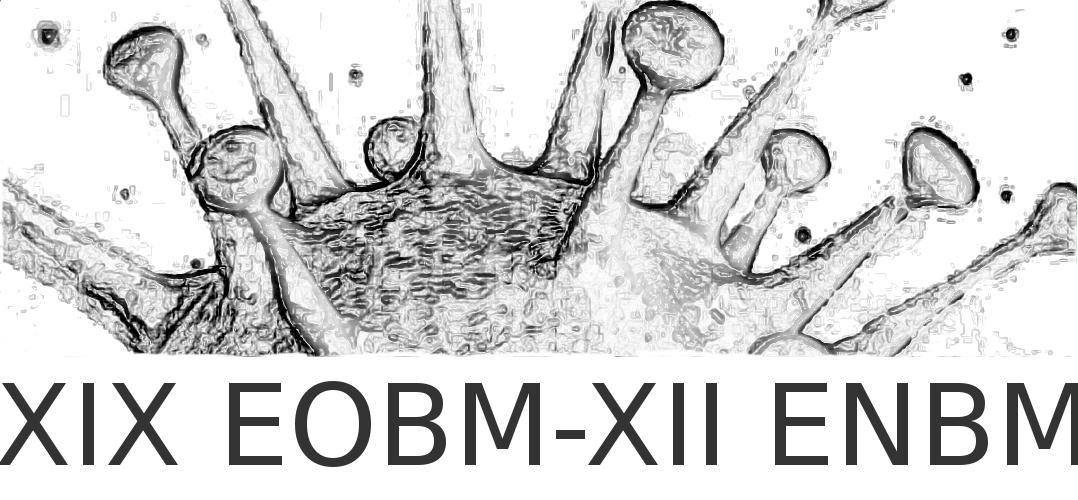
\includegraphics[height=1.0cm]{./figures/bar_background.png}
}
\metroset{block=fill}
%%%%%%%%%%%%%%%%%%%%%%%%%%%%%%%%%%%%%%%%%%%%%%%%%%%%%%%%%%%%%%%%%%%%%%%%%%%%%%%%
\def\Q#1#2{\frac{\partial #1}{\partial #2}}
\usetikzlibrary{arrows,shapes}
%%%%%%%%%%%%%%%%%%%%%%%%%%%%%%%%%%%%%%%%%%%%%%%%%%%%%%%%%%%%%%%%%%%%%%%%%%%%%%%%
%------------------------------------Theorems 
\theoremstyle{plain} % default
\newtheorem{Teorema}{Teorema}
\newtheorem{Ejemplo}{Ejemplo}
\theoremstyle{definition}
\newtheorem{Definicion}{Definici\'on}
\newtheorem{Corolario}{Corolario}
\newtheorem{Proposicion}{Proposici\'on}
\newtheorem{Prueba}{Prueba}
\theoremstyle{definition}
\newtheorem{definicion}{Definici\'on}
\newtheorem{lema}{Lema}
%-----------------------------ExtrasDeTercerPresentacion
%--------------------------------Fancyboxes-------------------------------------
\definecolor{myblue}{rgb}{.8, .8, 1}
\definecolor{shadecolor}{cmyk}{0,0,0.41,0}
\newcommand*\mybluebox[1]{%
	\colorbox{myblue}{\hspace{1em}#1\hspace{1em}}
}
\newcommand*\myyellowbox[1]{%
	\colorbox{darkyellow}{\hspace{1em}#1\hspace{1em}}
}
%--------------------------------------------------------------------------
\definecolor{shadecolor}{cmyk}{0,0,0.41,0}
\definecolor{light-blue}{cmyk}{0.25,0,0,0}
\newsavebox{\mysaveboxM} % M for math
\newsavebox{\mysaveboxT} % T for text
\newcommand*\Garybox[2][Example]{%
	\sbox{\mysaveboxM}{#2}%
		\sbox{\mysaveboxT}{\fcolorbox{black}{light-blue}{#1}}%
			\sbox{\mysaveboxM}{%
	\parbox[b][\ht\mysaveboxM+.5\ht\mysaveboxT+.5\dp\mysaveboxT][b]{%
		\wd\mysaveboxM}{#2}%
	}%
	\sbox{\mysaveboxM}{%
		\fcolorbox{black}{shadecolor}{%
		\makebox[\linewidth-10em]{\usebox{\mysaveboxM}}%
		}%
	}%
	\usebox{\mysaveboxM}%
	\makebox[0pt][r]{%
		\makebox[\wd\mysaveboxM][c]{%
			\raisebox{\ht\mysaveboxM-0.5\ht\mysaveboxT
			+0.5\dp\mysaveboxT-0.5\fboxrule}{\usebox{\mysaveboxT}}%
		}%
	}%
}
\newcommand\Fontvi{\fontsize{7}{7.2}\selectfont}
%%%%%%%%%%%%%%%%%%%%%%%%%%%%%%%%%%%%%%%%%%%%
\definecolor{kugreen}{RGB}{50,93,61}
\definecolor{kugreenlys}{RGB}{132,158,139}
\definecolor{kugreenlyslys}{RGB}{173,190,177}
\definecolor{kugreenlyslyslys}{RGB}{214,223,216}
\definecolor{greenArea}{RGB}{124,252,124}
\definecolor{hellmagenta}{rgb}{1,0.75,0.9}
\definecolor{hellcyan}{rgb}{0.75,1,0.9}
\definecolor{hellgelb}{rgb}{1,1,0.8}
\definecolor{colKeys}{rgb}{0,0,1}
\definecolor{colIdentifier}{rgb}{0,0,0}
\definecolor{colComments}{rgb}{1,0,0}
\definecolor{colString}{rgb}{0,0.5,0}
\definecolor{darkyellow}{rgb}{1,0.9,0}
\setbeamercovered{transparent}
\lstset{%
    language=[AlLaTeX]TEX,%
    float=hbp,%
    basicstyle=\ttfamily\small, %\usepackage{cir}
    identifierstyle=\color{colIdentifier}, %
    keywordstyle=\color{colKeys}, %
    stringstyle=\color{colString}, %
    commentstyle=\color{colComments}, %
    columns=flexible, %
    tabsize=3, %
    frame=single, %
    extendedchars=true, %
    showspaces=false, %
    showstringspaces=false, %
    numbers=left, %
    numberstyle=\tiny, %
    breaklines=true, %
    backgroundcolor=\color{hellgelb}, %
    breakautoindent=true, %
    captionpos=b,%
    xleftmargin=18pt,%
    xrightmargin=\fboxsep%
}
\pgfplotsset{
    left segments/.code={\pgfmathsetmacro\leftsegments{#1}},
    left segments=3,
    left/.style args={#1:#2}{
        ybar interval,
        domain=#1:#2,
        samples=\leftsegments+1,
        x filter/.code=\pgfmathparse{\pgfmathresult}
       }
}
\DeclareMathOperator{\sign}{sgn}
\newcommand{\innerprod}[2]{\left\langle#1, #2\right\rangle}
\newcommand\bound{10} % bound number of points on each side of N
\newcommand\labelnum[3][]{
	\begin{scope}[font=\footnotesize,x=.3cm,#1]
	  \foreach \mypt in {0,#2,...,\bound}{
	    \draw(\mypt,0)circle[radius=2pt];
	    \draw(-\mypt,0)circle[radius=2pt];
	  }
	  \draw(-\bound-5,0)--(\bound+5,0) node[pos=0, left]{$t$};
	  \node(start)[at={(-\bound-4,0)},label=below:{$t_0=0$}]{$[$};
	  \node(end)[at={(\bound+4,0)},label=below:{$T=Nh$}]{$]$};
	  \node[%
		  at={($(start)!.319!(end)$)},
		  label=below:{
			   $\underbrace{}_{h}$
			}%
			]{\vphantom{$[$}};
	  \node[at={($(start)!.57!(end)$)},label=below:{$t_{n+1}$}]{\vphantom{$[$}};
	  \filldraw(0,0)circle[radius=2pt];
	  \node[at={(-\bound-2,0)},above]{$\cdots$};
	  \node[at={(\bound+2,0)},above]{$\cdots$};
	  \node[at={(0,0)},above=5pt]{#3};
	\end{scope}
}
\tcbuselibrary{skins,breakable}

\defaultbibliography{CharlaBib}
\defaultbibliographystyle{abbrv}
\begin{document}
	\maketitle
 	\section*{Introducción}
		%
%
% Esta parte funciona con Okular bajo linux.
% Para Windows, comentar el siguiente bloque y
% habilitar lo que sigue y presentar con acrobad reader
%
%
%
% %%%%%%%%%%%%%%%%%%%%%%%%%%%%%%%%%%%%%%%%%%%%%%%%%%
\begin{frame}{Proceso de Remodelación en BMU}
	\begin{tikzpicture}[remember picture,overlay]
	  \node[anchor=south west, inner sep=0pt] at (current page.south west) {%
    \movie[%
	    height = \paperheight,%
	    width = \paperwidth,%
	    poster,%
			showcontrols]{}{./Video/oc-ob.mp4}%
      };
  \end{tikzpicture}
\end{frame}
%%%Para windows (guacala!!!) es un purrun con el acrobad reader%%%
%\begin{frame}{Proceso de Remodelación en BMU}
%	\includemedia[
%	width=1\linewidth,height=0.6\linewidth,
%	activate=pageopen,
%	addresource=oc-ob.flv,        %adjust
%	flashvars={source=oc-ob.flv}  %adjust
%	]{\frame{Click!}}{VPlayer9.swf}
%\end{frame}
		%%%%%%%%%%%%%%%%%%%%%%%%%%%%%%%%%%%%%%%%%%%%%%%%%%%%%%%%%%%%%%%%5
\begin{frame}
	\frametitle{Fases de remodelación}
		\only<1-2>{%
			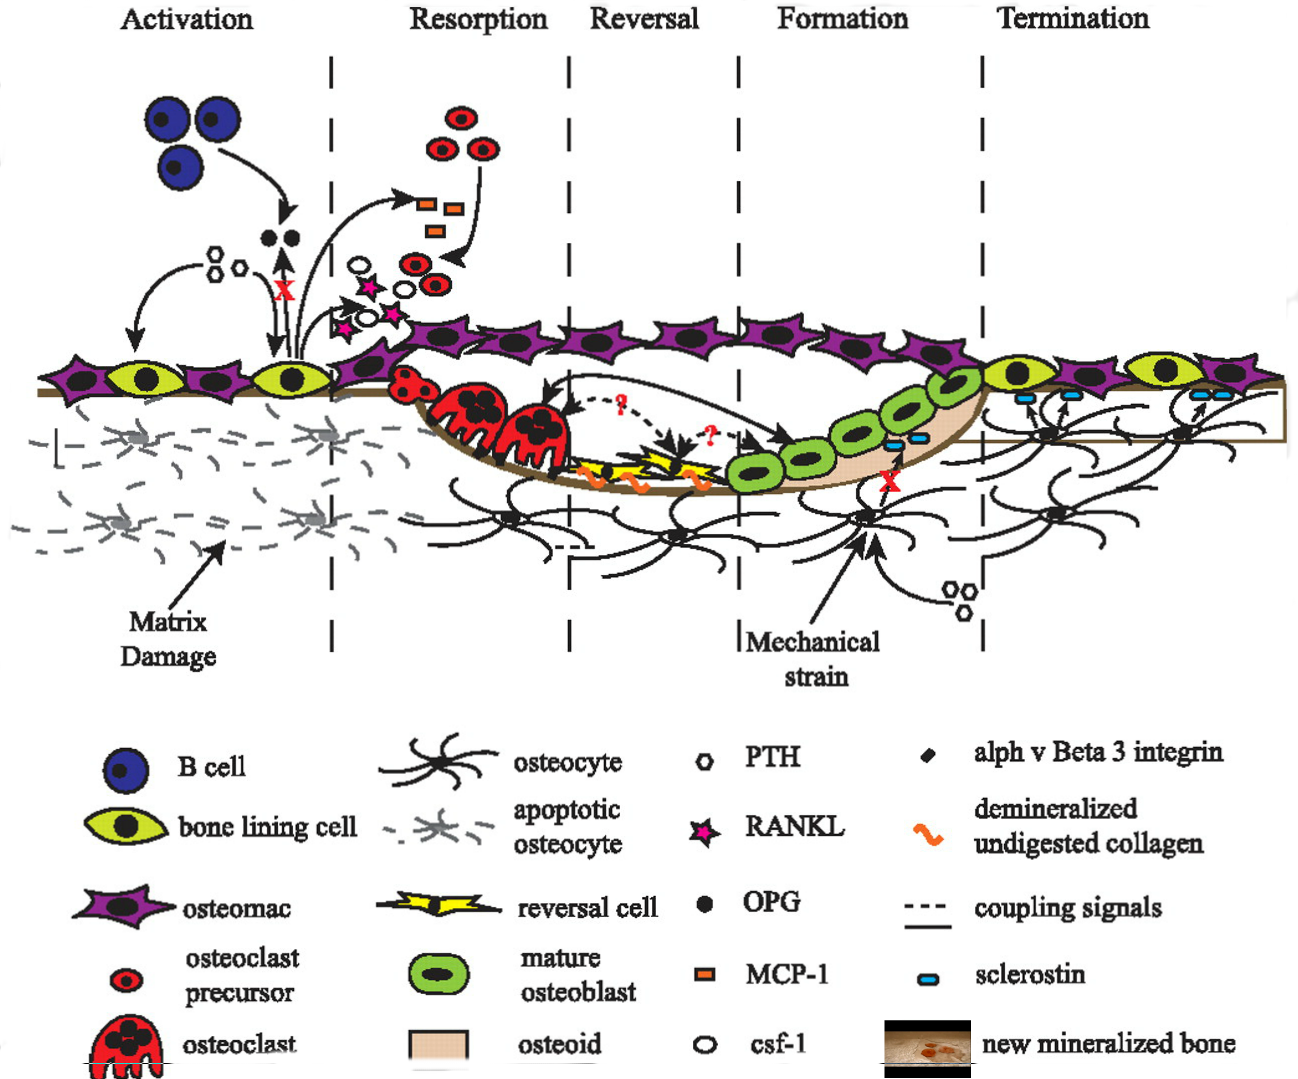
\includegraphics[width=\textwidth,keepaspectratio]{%
			./IMAGES/Komarova/boneRemodeling.png%
			}
		}
		\only<3-4>{%
			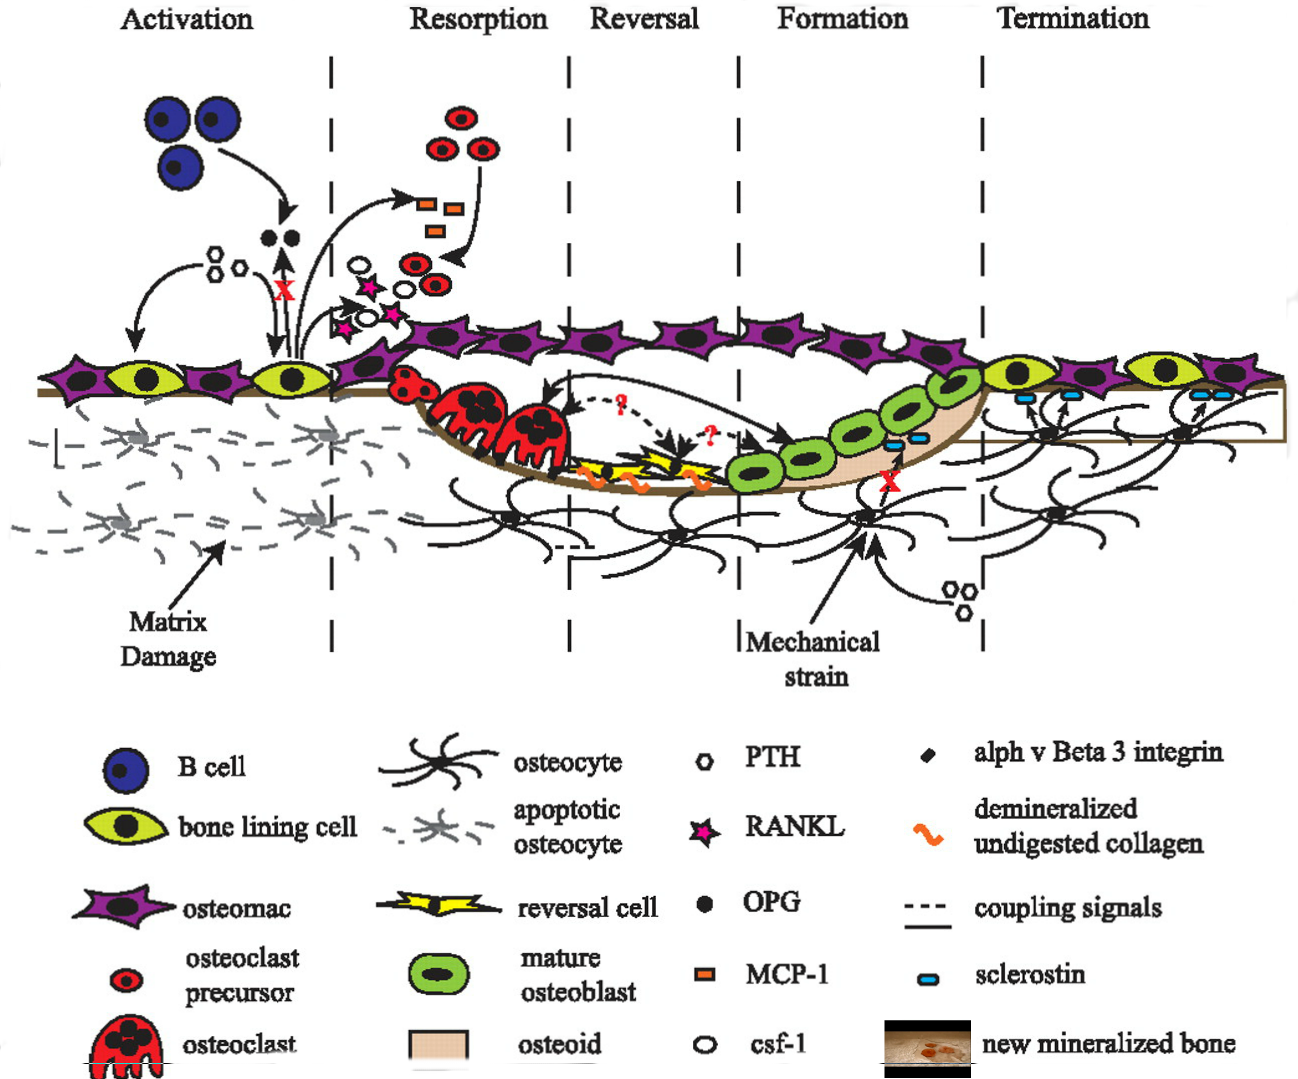
\includegraphics[width=.9\textwidth,keepaspectratio]{%
			./IMAGES/Komarova/boneRemodeling.png%
			}
		}

 		\only<1-2>{
			\begin{textblock*}{105mm}(10mm, 70mm)
				\begin{block}{Fases del proceso de remodelación}
						\begin{bibunit}[apalike]
						\nocite{Raggatt2010}
						\putbib
					\end{bibunit}
				\end{block}
			\end{textblock*}
 		}
\end{frame}

		\begin{frame}{}
	\frametitle{El Modelo de Komarova}
 	\only<1->{
		\begin{textblock*}{40mm}(10mm, 20mm)
			\begin{align*}
 			\frac{du}{dt} &=
 				u^{\kappa_1}
				\left(
					\alpha_1 v^{\gamma_1} - \beta_1
				\right)
				\\
			\frac{dv}{dt} &=
				v^{\kappa_2}
				\left(
					\alpha_2 u^{\gamma_2} - \beta_2
				\right)
			\\
			\only<3->{
					\frac{dz}{dt} &=
				-
				k_1 \max\{u - \widetilde{u}, 0\}
				\\
				&
				+
				k_1 \max\{v - \widetilde{v}, 0\}
			}
				\end{align*}
		\end{textblock*}
 	}
	\only<4>{% modelote
		\begin{textblock*}{.9\textwidth}(10mm, 5mm)
			\begin{exampleblock}{Descripción}
				\includegraphics[width=.98\textwidth, keepaspectratio]%
				{./IMAGES/Komarova/komarovaModelDescripcion.png}
			\end{exampleblock}
		\end{textblock*}	
	}
	\only<5>{% modelote
		\begin{textblock*}{.9\textwidth}(10mm, 5mm)
			\begin{exampleblock}{Descripción}
				\includegraphics[width=.98\textwidth, keepaspectratio]%
				{./IMAGES/Komarova/komarovaModelDescripcionb.png}
			\end{exampleblock}
		\end{textblock*}	
	}
	%
	\only<6>
	{
		\begin{textblock*}{.5\textwidth}(60mm, 20mm)
			\includegraphics[width=\textwidth, keepaspectratio]%
			{./IMAGES/Komarova/komarovaModel1.png}
		\end{textblock*}
	}
	\only<2-4>{
		\begin{textblock*}{100mm}(10mm, 63mm)
			\begin{bibunit}[alpha]
				\nocite{Komarova2003}
				%\biblio{CharlaBib.bib}
				\putbib
		  \end{bibunit}
  \end{textblock*}
	}
\end{frame}

		\begin{frame}{}
	\frametitle{Simplificación}
 	\only<1->{
		\begin{textblock*}{40mm}(10mm, 20mm)
			\begin{align*}
				\only<1>{
					\frac{du}{dt} &=
						u^{\kappa_1}
						\left(
							\alpha_1 v^{\gamma_1} - \beta_1
						\right)
						\\
					\frac{dv}{dt} &=
						v^{\kappa_2}
						\left(
							\alpha_2 u^{\gamma_2} - \beta_2
						\right)
					\\
 				}
				\only<2>{
					\frac{du}{dt} &=
					u^{
						\xcancel{\kappa_1}
					}
					\left(
						\alpha_1 v^{\gamma_1} - \beta_1
					\right)
					\\
				\frac{dv}{dt} &=
					v^{
						\xcancel{\kappa_2}
					}
					\left(
						\alpha_2 u^{\gamma_2} - \beta_2
					\right)
				\\
				}
				\only<3->{
					\frac{du}{dt} &=
					u
					\left(
						\alpha_1 v^{\gamma_1} - \beta_1
					\right)
					\\
				\frac{dv}{dt} &=
					v
					\left(
						\alpha_2 u^{\gamma_2} - \beta_2
					\right)
				\\
				} 			
				\only<5->{
						\frac{dz}{dt} &=
					-
					k_1 \max\{u - \widetilde{u}, 0\}
					\\
					&
					+
					k_1 \max\{v - \widetilde{v}, 0\}
				}
				\end{align*}
		\end{textblock*}
 	}
	\only<4>{% modelote
		\begin{textblock*}{1.2\textwidth}(0mm, 0mm)
			\includegraphics[width=\textwidth, keepaspectratio]%
			{./IMAGES/Komarova/silviaModelDescripcion.png}
		\end{textblock*}	
	}
%
	\only<6>
	{
		\begin{textblock*}{.5\textwidth}(60mm, 15mm)
			\includegraphics[width=\textwidth, keepaspectratio]%
			{./IMAGES/Komarova/silviaModel1.png}
		\end{textblock*}
	}
	\only<7>
	{
		\begin{textblock*}{.5\textwidth}(60mm, 15mm)
			\includegraphics[width=\textwidth, keepaspectratio]%
			{./IMAGES/Komarova/silviaModel2.png}
		\end{textblock*}
	}
	
	
	\only<3->{
		\begin{textblock*}{100mm}(10mm, 65mm)
			\begin{bibunit}[alpha]
				\nocite{Jerez2015a}
				\putbib
		  \end{bibunit}
  \end{textblock*}
	}
\end{frame}

		\begin{frame}
	\frametitle{Objetivo}
	\begin{alertblock}{Objetivo}
		\textbf{Ilustrar} cómo incorporar \textbf{incertidumbre} con una 
		perturbación estocástica.
	\end{alertblock}
\end{frame}

 	%\section{}
%%%%%%%%%%%%%%%%%%%%%%%%%%%%%%%%%%%%%%%%%%%%%%%%%%%%%%%%%%%%%%%%%%%%%%%%%%%%%%%%
	\begin{frame}{Esquema de Charla}
   		\setbeamertemplate{section in toc}[sections numbered]
   		\tableofcontents[hideallsubsections]
 	\end{frame}
 	\section{Perturbación estocástica}
		\begin{frame}
	\frametitle{¿Por qué incorporar incertidumbre a un modelo?}
	\begin{textblock*}{37mm}(3mm, 10mm)
		\begin{block}{Efectos Ambientales}
			\begin{itemize}
				\item \textcolor<2-3>{orange}{Extinción}
				\item \textcolor<4>{orange}{Epidemias}
			\end{itemize}
		\end{block}
	\end{textblock*}
	\begin{textblock*}{75mm}(45mm, 10mm)
		\begin{alertblock}{%
				\only<2>{%
					Ruido ambiental suprime extinción%
				}%
				\only<3>{%
					Color (correlación) induce extinción
				}%
				\only<4>{%
					$\mathcal{R}_0$: endémico g.a.e $\to$ osc. per 
					%$\mathcal{R}_0$ (determinista)
				}%
		}%Block titles
			\only<2>{
				\begin{bibunit}[apalike]
					\nocite{Mao2002}
					\putbib
			  \end{bibunit}
			}
			\only<3>{
				\begin{bibunit}[apalike]
					\nocite{Ripa1996}
					\putbib
			  \end{bibunit}
			}
			\only<4>{
				\begin{bibunit}[apalike]
					\nocite{Allen2013}
					\putbib
			  \end{bibunit}
			}
		 \end{alertblock}
	\end{textblock*}
\end{frame}
		\begin{frame}
	\frametitle{Alternativas}
	\begin{textblock*}{37mm}(3mm, 10mm)
		\begin{block}{Efectos Ambientales}
			\begin{itemize}
				\item Extinción
				\item Epidemias
			\end{itemize}
		\end{block}
	\end{textblock*}
%%%%%%%%%%%%%%%%%%%%%%%%%%%%%%%%%%%%%%%%%%%%%%%%%%%%%%%%%%%%%%%%%%%%%%%%%%%%%%%
	\begin{textblock*}{37mm}(3mm, 35mm)
		\begin{block}{En biología}
			\begin{itemize}
				\item<2> \textcolor<2>{orange}{CTMCs}
				\item<3-4,6>\textcolor<3-4,6>{orange}{
					\textbf<6>{%
						Perturbación de parámetros
					}
				}
				\item<5> \textcolor<5>{orange}{Procesos reversibles en media}
			\end{itemize}
		\end{block}
	\end{textblock*}
%%%%%%%
	\begin{textblock*}{75mm}(45mm, 35mm)
		\begin{alertblock}{%
				\only<2>{%
					$\mathbf{MC}+\mathbf{ME}$ $\to$ $SDE$%
				}%
				\only<3,6>{%
					$\varphi dt \rightsquigarrow \varphi dt+ \sigma dB_t$%
				}%
				\only<4>{%
					$\varphi dt \rightsquigarrow \varphi dt+F(x)dB_t$%
				}%
				\only<5>{%
					$d \varphi_t = (\varphi_e -\varphi_t)dt + \sigma_\varphi dBt$ %
				}%
		}%Block titles
			\only<2>{
				\begin{bibunit}[apalike]
					\nocite{Allen2017}
					\putbib
			  \end{bibunit}
			}
			\only<3>{
				\begin{bibunit}[apalike]
					\nocite{Gray2011}
					\putbib
			  \end{bibunit}
			}
			\only<4>{
				\begin{bibunit}[apalike]
					\nocite{Schurz2015}
					\putbib
			  \end{bibunit}
			}
			\only<5>{
				\begin{bibunit}[apalike]
					\nocite{Allen2016}
					\putbib
			  \end{bibunit}
			}
		 \end{alertblock}
	\end{textblock*}
\end{frame}


		\begin{frame}
	\frametitle{Pertrubación}
	\begin{textblock*}{40mm}(10mm, 20mm)
		\begin{align*}
			\only<1->{
				\frac{du}{dt} &=
					u
					\left(
						\alpha_1 v^{\gamma_1} - \beta_1
					\right)
						\\
				\frac{dv}{dt} &=
					v
					\left(
						\alpha_2 u^{\gamma_2} - \beta_2
					\right)
				\\
			}
		\end{align*}
	\end{textblock*}
	\begin{textblock*}{40mm}(10mm, 45mm)
		\begin{align*}
			\only<2->{
				du &=
					\alpha_1 u v^{\gamma_1} dt
					 - 
					 u\beta_1 dt
						\\
				dv &=
					\alpha_2 u^{\gamma_2} v dt
					- 
					v\beta_2 dt
				\\
			}
		\end{align*}
	\end{textblock*}
	\begin{textblock*}{40mm}(10mm, 65mm)
		\begin{align*}
			\only<3->{
				\beta_i dt \rightsquigarrow
				\beta_i dt 
				+ 
				\textcolor{orange}{
					\sigma_i dB_i(t)
				}
				\\
			}
		\end{align*}
	\end{textblock*}
%%%%%%%%%%%%%%%%%%%%%%%%%%%%%%%%%%%%%%%%%%%%%%%%%
	\only<4->{
		\begin{textblock*}{65mm}(60mm, 37mm)
			\begin{alertblock}{Nuevo Modelo}
				\begin{align*}
					du_t &=
						u_t
						\left(
							\alpha_1 v_t^{\gamma_1} - \beta_1
						\right) 
						dt
						+
						\textcolor{orange}{
							\sigma_1 u_t dB_1(t)
						}
						\\
					dv_t &=
						v_t
						\left(
							\alpha_2 u_t^{\gamma_2} - \beta_2
						\right)
						dt
						+
						\textcolor{orange}{
							\sigma_2 v_t dB_2(t)
						}
				\end{align*}
			\end{alertblock}
		\end{textblock*}
	}
\end{frame}
%%%%%%%%%%%%%%%%%%%%%%%%%%%%%%%%%%%%%%%%%%%%%%%%%


 	\section{Propiedades de la solución}
		\begin{frame}[plain]
	\frametitle{Existe, única y positiva}
	 \begin{textblock*}{40mm}(10mm, 10mm)
		 \begin{enumerate}[(H-1)]
		  \item<2->  $\gamma_1<0$, $\gamma_2>0$,
		  \item<2->  $|\gamma_1|\leq\gamma_2$ ,
		  \item<2->  $\alpha_1\gamma_2\leq\alpha_2|\gamma_1|,$
			\item<5-6> $-1< \gamma_1 < 0$ and $0<\gamma_2< 1$, 
			\item<5-6> $ \exists p>1$ t.q
						$\beta_i>\frac{1}{2}p(p-1)\sigma_i$
		 \end{enumerate}
	\end{textblock*}
	%%%%%%%%%%%
	\only<3->{%ecuación
		\begin{textblock*}{65mm}(60mm, 10mm)
					\begin{align*}
						du_t &=
							u_t
							\left(
								\alpha_1 v_t^{\gamma_1} - \beta_1
							\right) 
							dt
							+
							\textcolor{orange}{
								\sigma_1 u_t dB_1(t)
							}
							\\
						dv_t &=
							v_t
							\left(
								\alpha_2 u_t^{\gamma_2} - \beta_2
							\right)
							dt
							+
							\textcolor{orange}{
								\sigma_2 v_t dB_2(t)
							}\\
						x_t&=(u_t,v_t)
					\end{align*}
		\end{textblock*}
	}
	\only<4->{%
		\begin{textblock*}{47mm}(10mm, 55mm)
		\begin{Teorema}
			$\forall$ $(u_0,v_0)$ positivos,
			$\exists !$  $(u_t,v_t)$ continua e invariante 
			$\in\mathbb{R}^2_+$
			(c.p.1.).
		\end{Teorema}
	\end{textblock*}
	}
%
	\only<6->{
		\begin{textblock*}{47mm}(65mm, 55mm)
			\begin{Teorema}[a.l.p.]
				 $\forall \epsilon>0$, %
				 $\exists K(\epsilon)<\infty$ %
				 t.q. % 
				 $\displaystyle
				  \limsup_{t \to \infty}
					  \probX{|x_t|\geq K} \leq\epsilon
				 $.%
			\end{Teorema}
	\end{textblock*}
	}%
	%%%%%%%%%%%%%%%%%%%%%%%%%%%%%%%%%%%%%
	\only<7>{
		\begin{textblock*}{110mm}(10mm, 35mm)
			\begin{Teorema}[oscilaciones]
				\begin{align*}
				 \limsup_{t \to \infty} u_t
					 &\geq \xi_2,
					 &
					 \limsup_{t \to \infty} v_t
					 &\geq\xi_1,
					 &  c.s.
				\\
				 \liminf_{t \to \infty} u_t
					 &\leq\xi_2,
					 &
					 \liminf_{t \to \infty} v_t
					 &\leq\xi_1,
					 & c.s.
				\\
				\xi_1
					&=
					\left(
						\frac{\beta_1+\frac{1}{2}\,\sigma_1^2}{\alpha_1}
					\right)^{\frac{1}{\gamma_1}
					},
					&
					\xi_2
					&=
					\left(
						\frac{\beta_2+\frac{1}{2},\sigma_2^2}{\alpha_2}
					\right)^{\frac{1}{\gamma_2}}.
				\end{align*}
			\end{Teorema}
		\end{textblock*}
	}
\end{frame}

 	\section{Resultados numéricos}
		%%%%%%%%%%%%%%%%%%%%%%%%%%%%%%%%%%%%%%%%%%%%%%%%%
\begin{frame}[plain]	
	\begin{columns}
		\column[t]{60mm}
			%\begin{tikzpicture}[remember picture,overlay]
% 			\node[anchor=south west, inner sep=0pt] at (%
% 				current page.south west) {%
 			\movie[%
				height = \textwidth,,%
				width = 1.1\textwidth,%
				poster,%
				%keepaspectratio,
				showcontrols]{}{./Video/StoPLBRM.mp4}%
% 				};
% 		\end{tikzpicture}
		%\end{textblock*}
		\column[t]{50 mm}
		%\begin{textblock*}{.5\textwidth}(65mm, 20mm)
				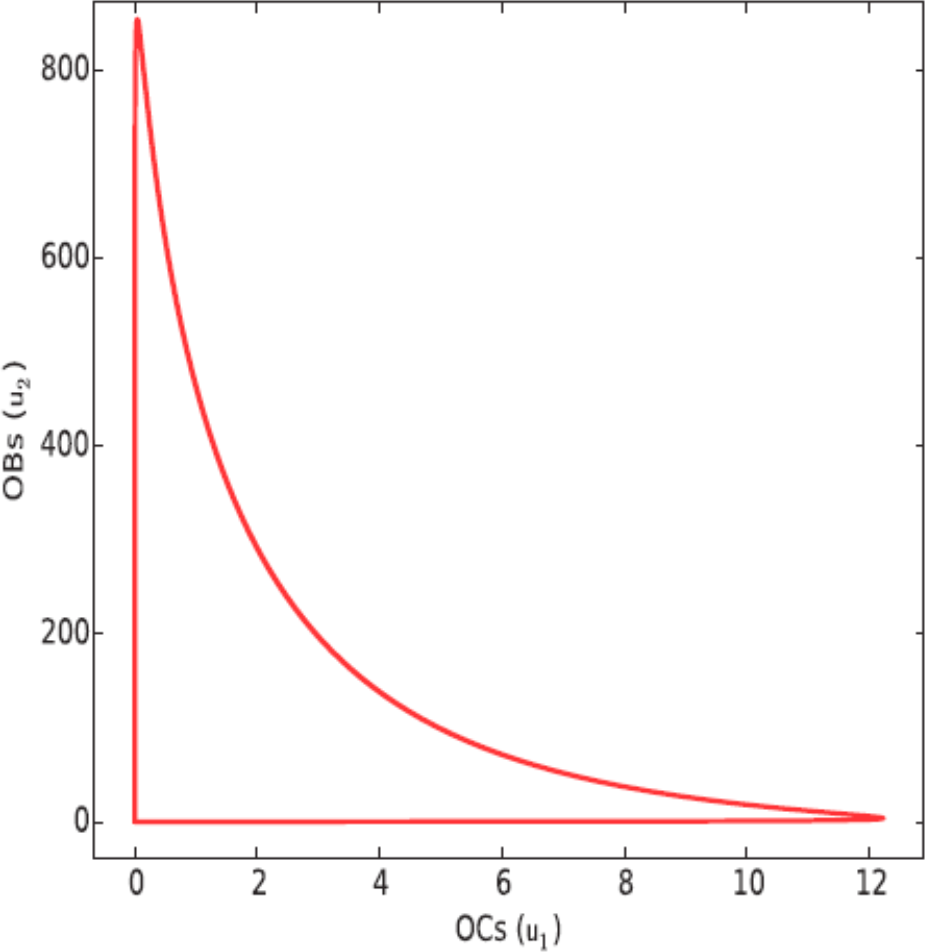
\includegraphics[width=.9\textwidth, keepaspectratio]{%
					./IMAGES/ComparacionDeModelos/pfSilvia.png}
		%\end{textblock*}	
	\end{columns}	
\end{frame}
%%%%%%%%%%%%%%%%%%%%%%%%%%%%%%%%%%%%%%%%%%%%%%%%%%%%%%%%%%%%%%%
\begin{frame}[plain]{Comparación de Fases}
	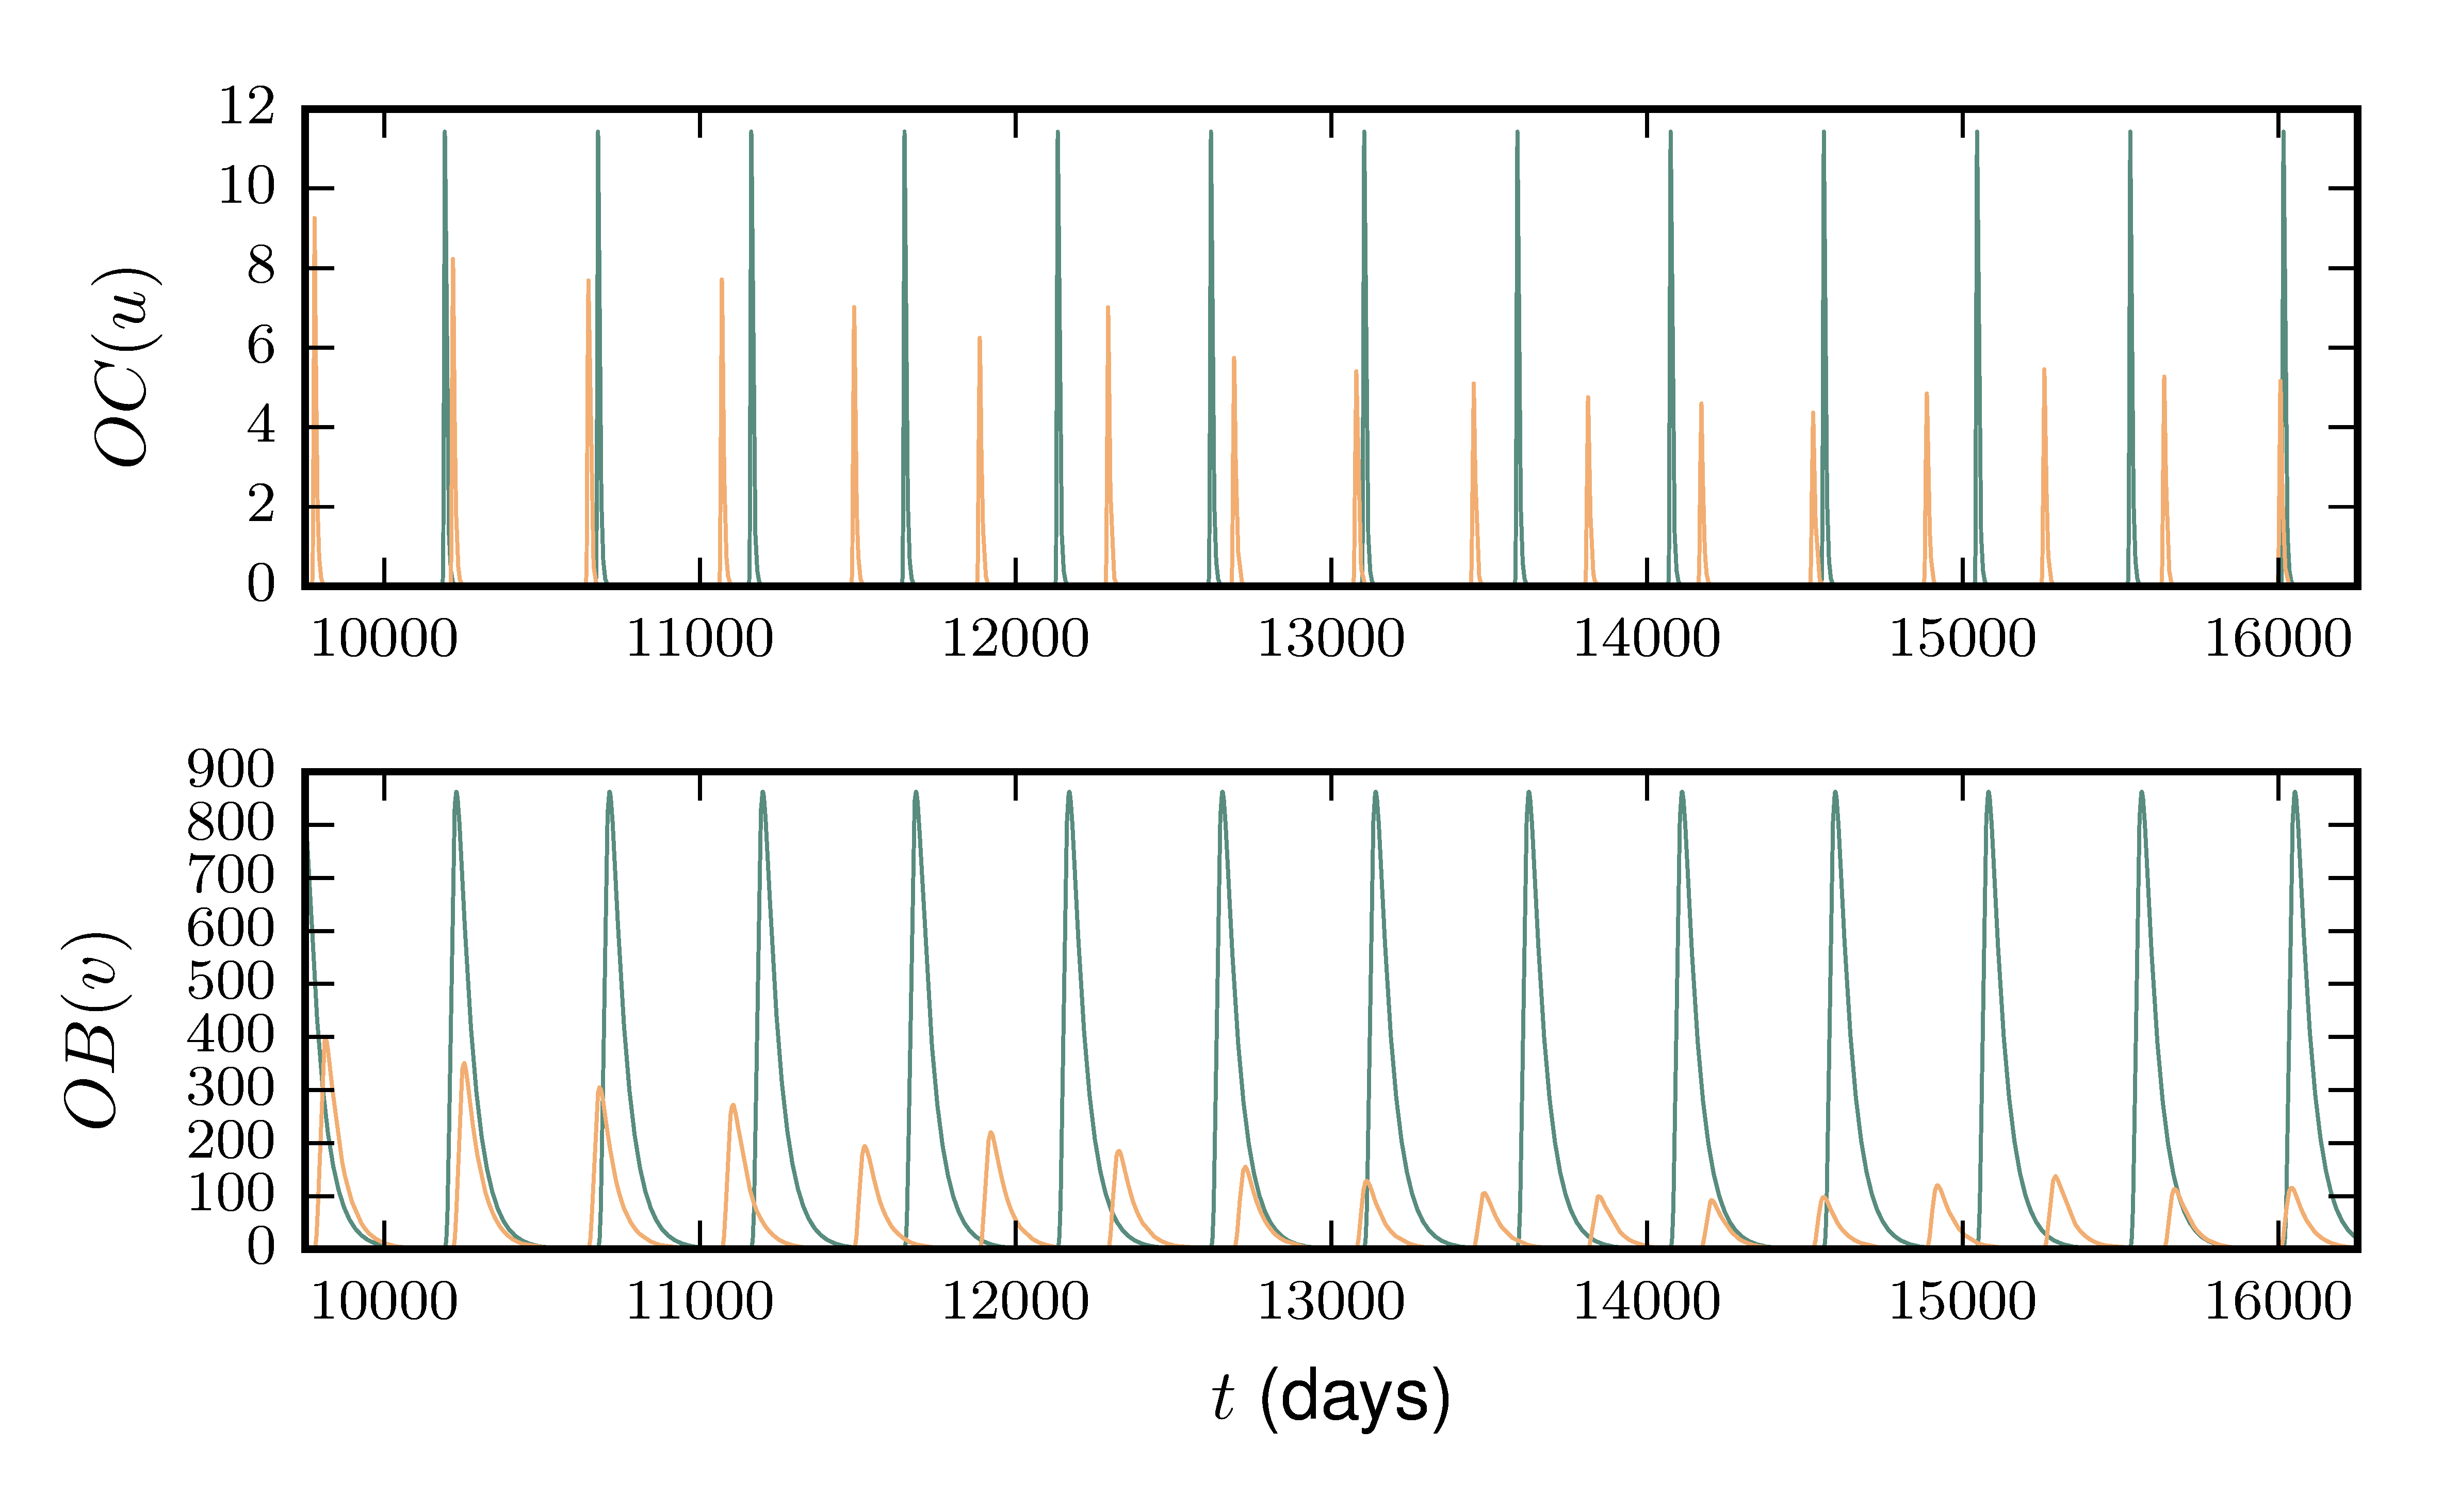
\includegraphics[width=\textwidth,keepaspectratio]{%
		./IMAGES/LongShortTime/ComparacionDeFase.png}
\end{frame}
%%%%%%%%%%%%%%%%%%%%%%%%%%%%%%%%%%%%%%%%%%%%%%%%%%%%%%%%%%%%%%%
\begin{frame}[plain]{PF tiempo corto (7 años) vs timpo largo (80-90 años)} 
	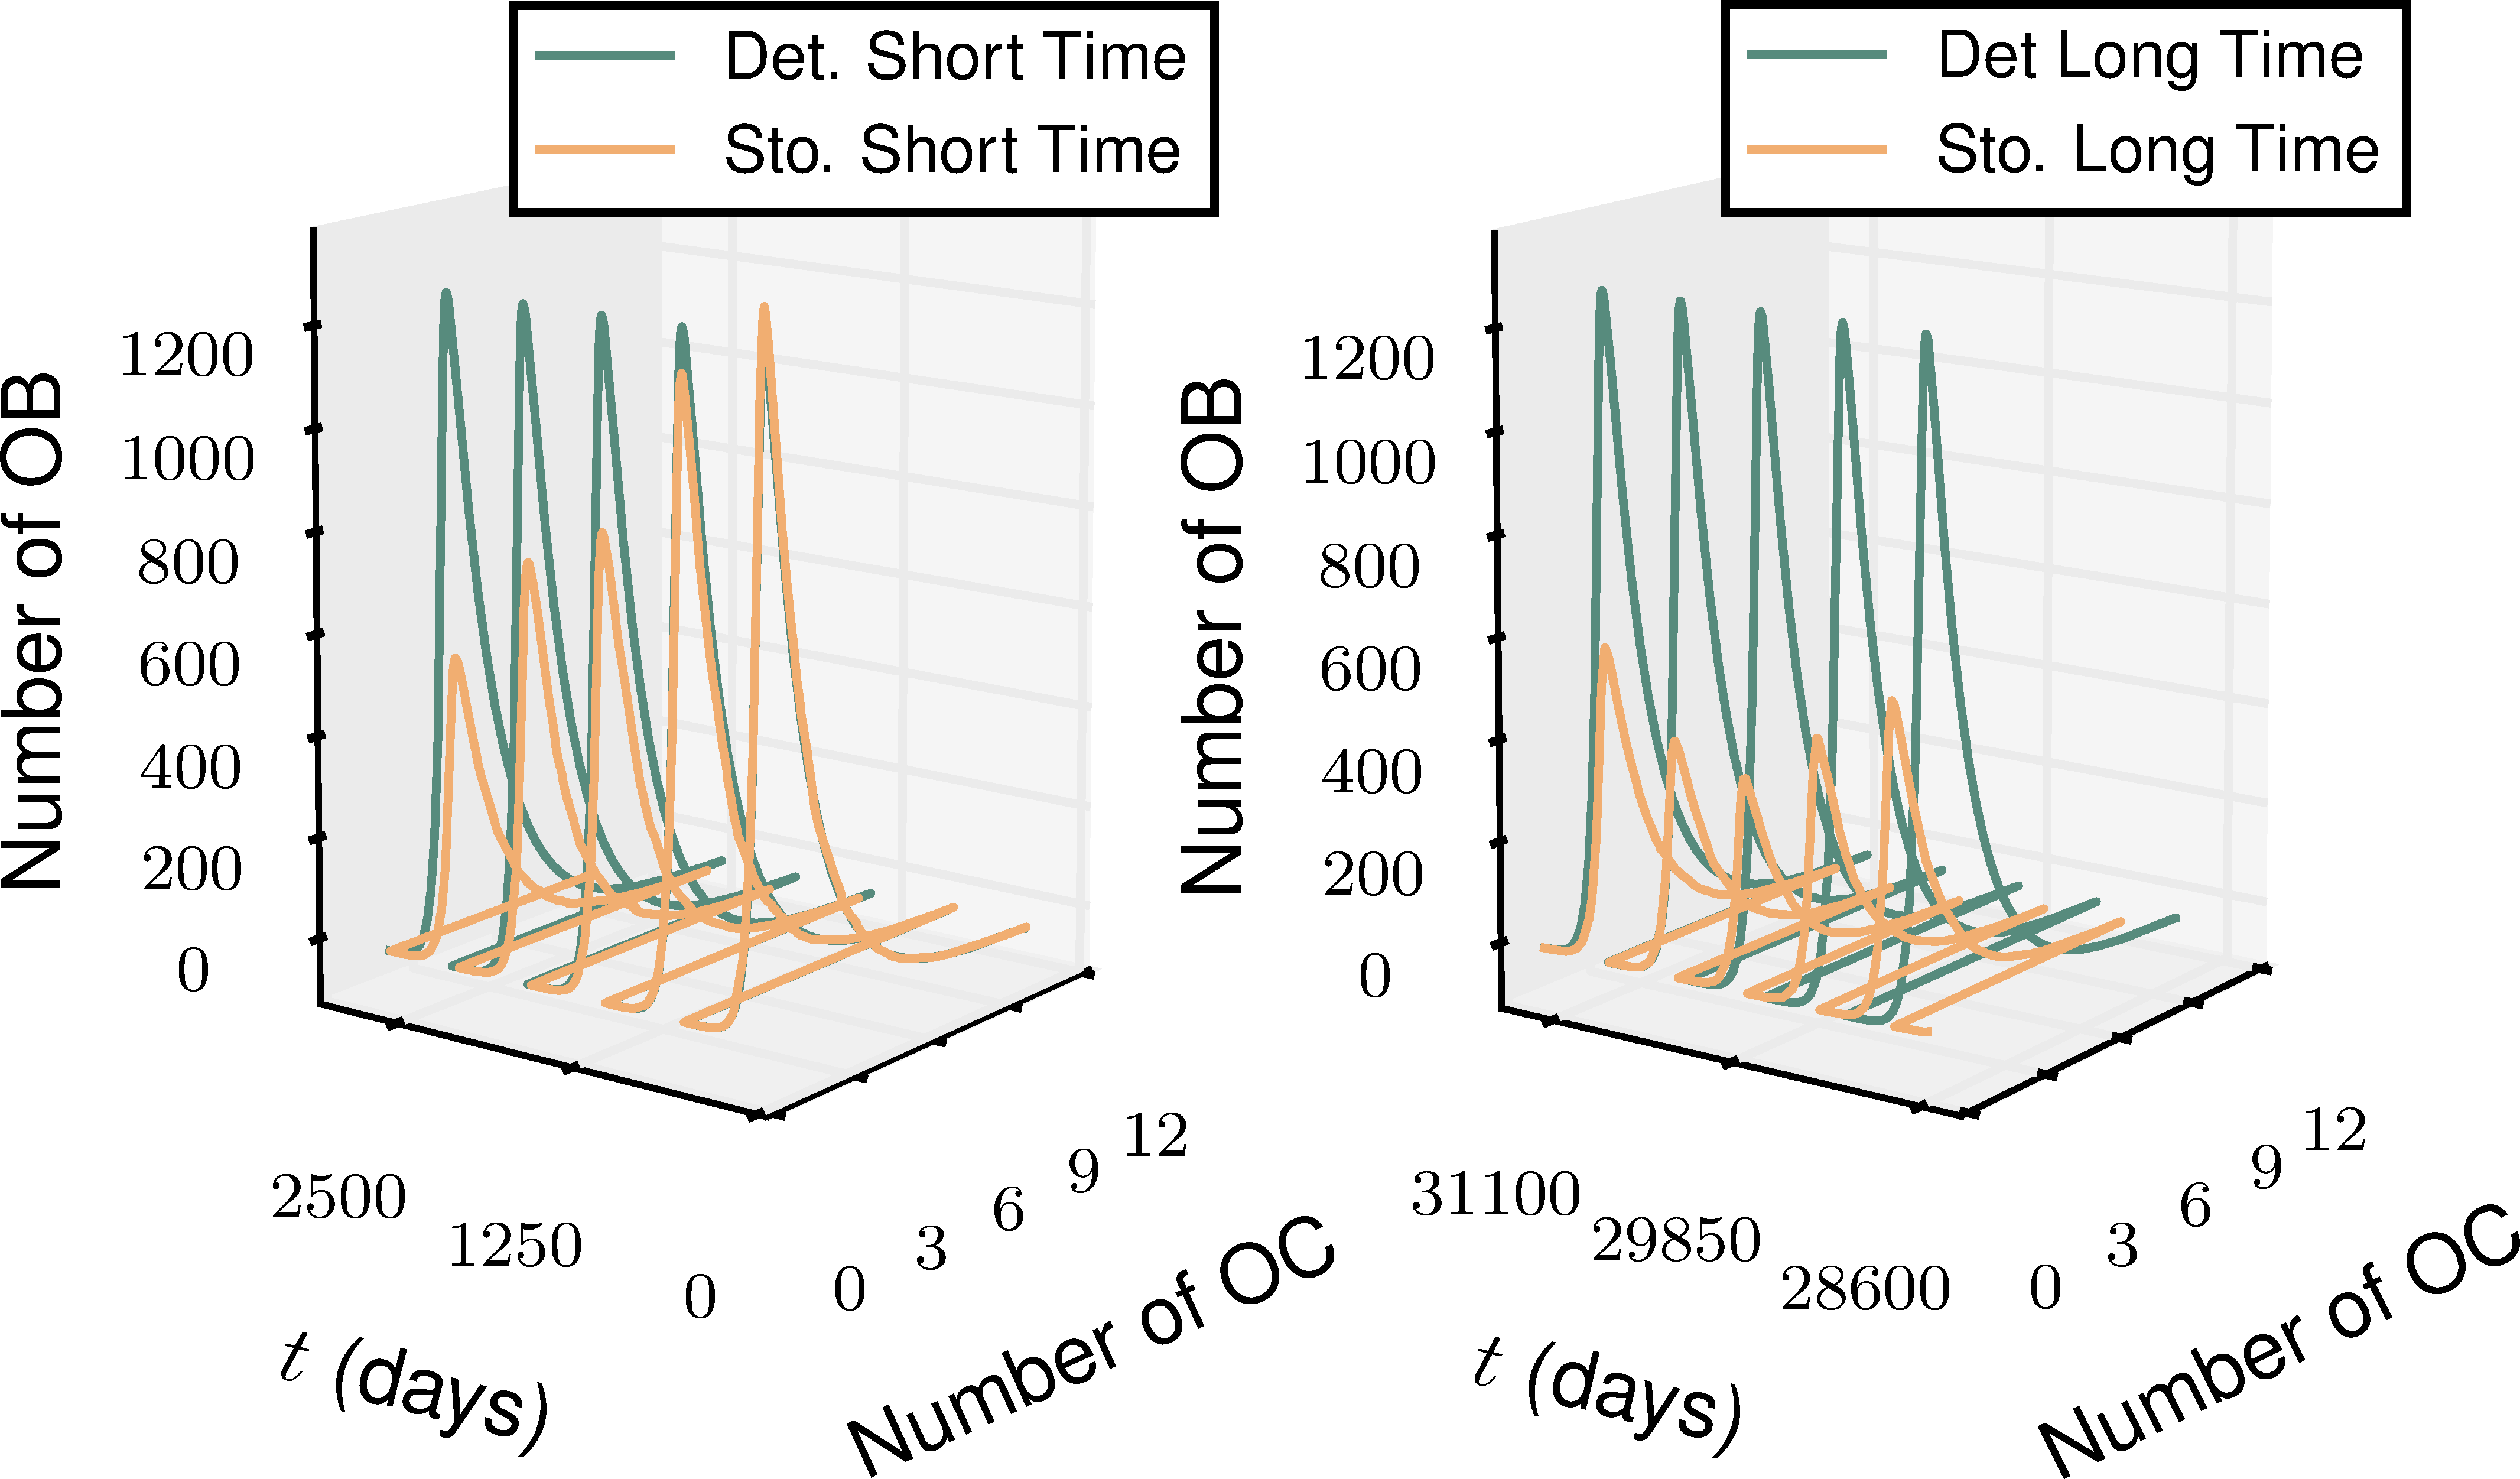
\includegraphics[width=\textwidth,keepaspectratio]{%
		%./IMAGES/LongShortTime/PhasePotrait3d(a).png
		./IMAGES/LongShortTime/ComparacionDePlanosFase.png%
		}
\end{frame}
%%%%%%%%%%%%%%%%%%%%%%%%%%%%%%%%%%%%%%%%%%%%%%%%%%%%%%%%%%%%%%%
\begin{frame}[plain]{Oscilaciones en torno a $\xi_i$}
	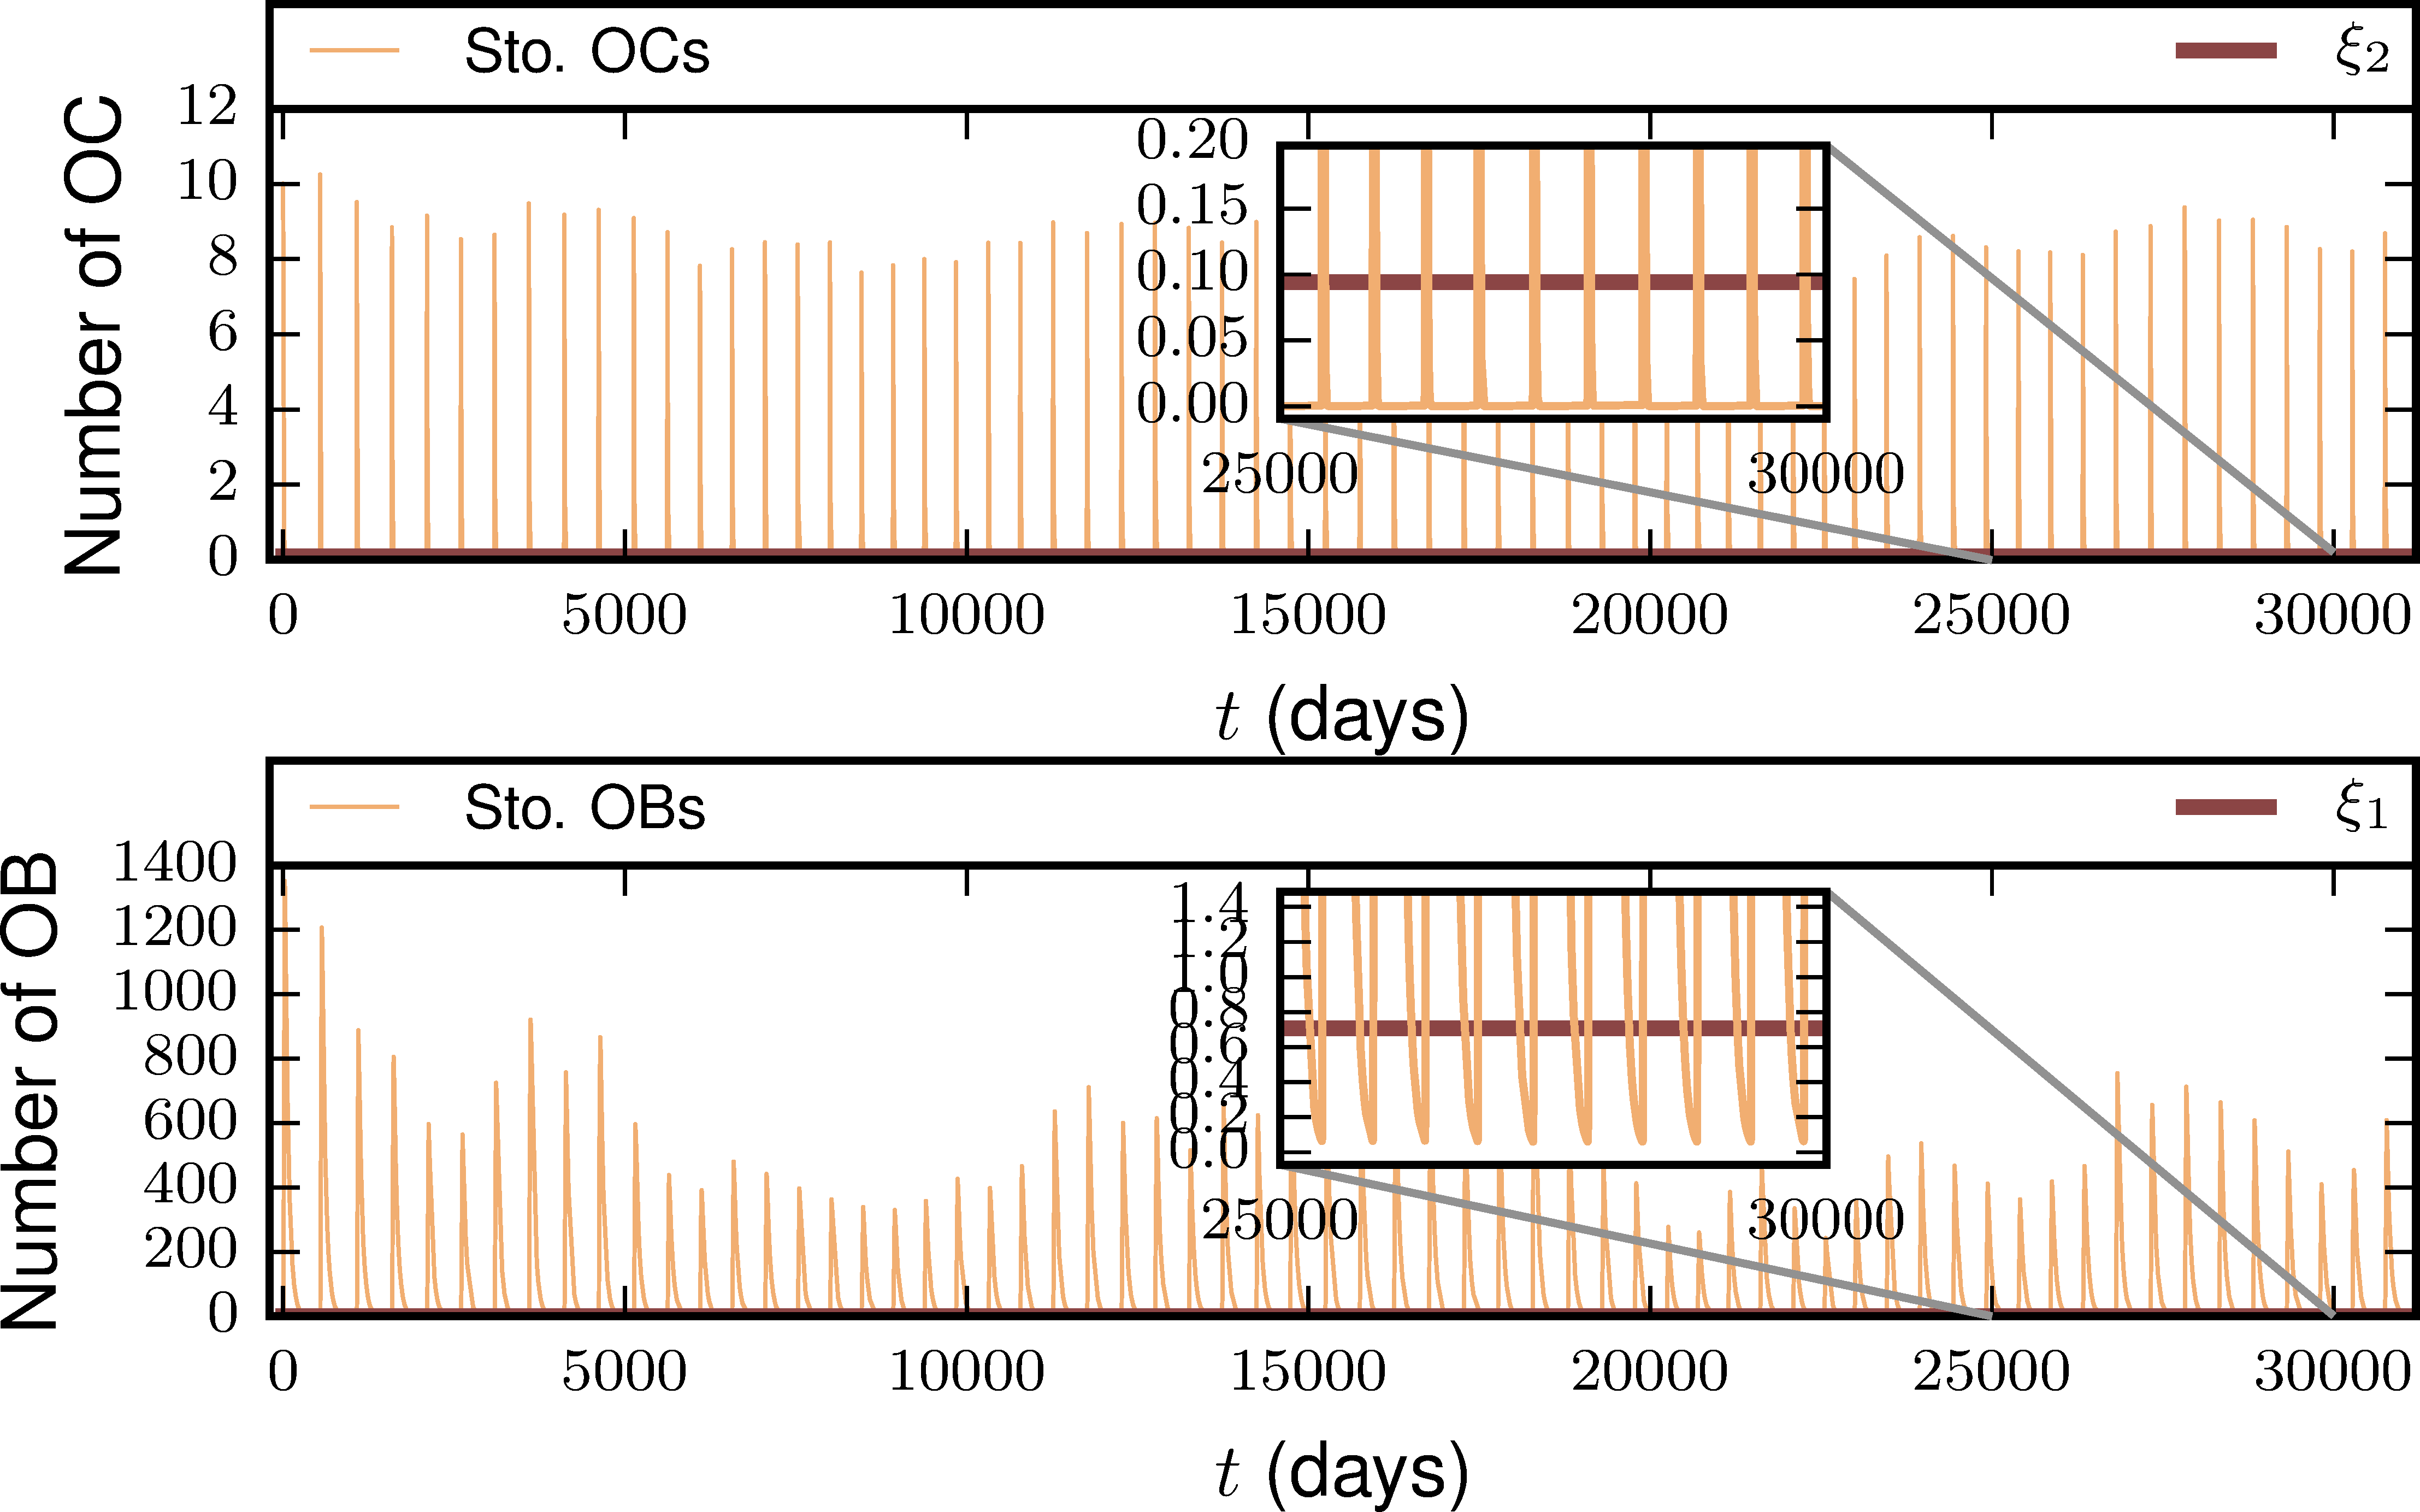
\includegraphics[width=\textwidth,keepaspectratio]{%
		%./IMAGES/LongShortTime/PhasePotrait3d(b).png
		./IMAGES/LongShortTime/OscilacionesXi1Xi2.png%
		}
\end{frame}
%%%%%%%%%%%%%%%%%%%%%%%%%%%%%%%%%%%%%%%%%%%%%%%%%%%%%%%%%%%%%%%
\begin{frame}[plain]{Trayectoria larga y  masa osea}
	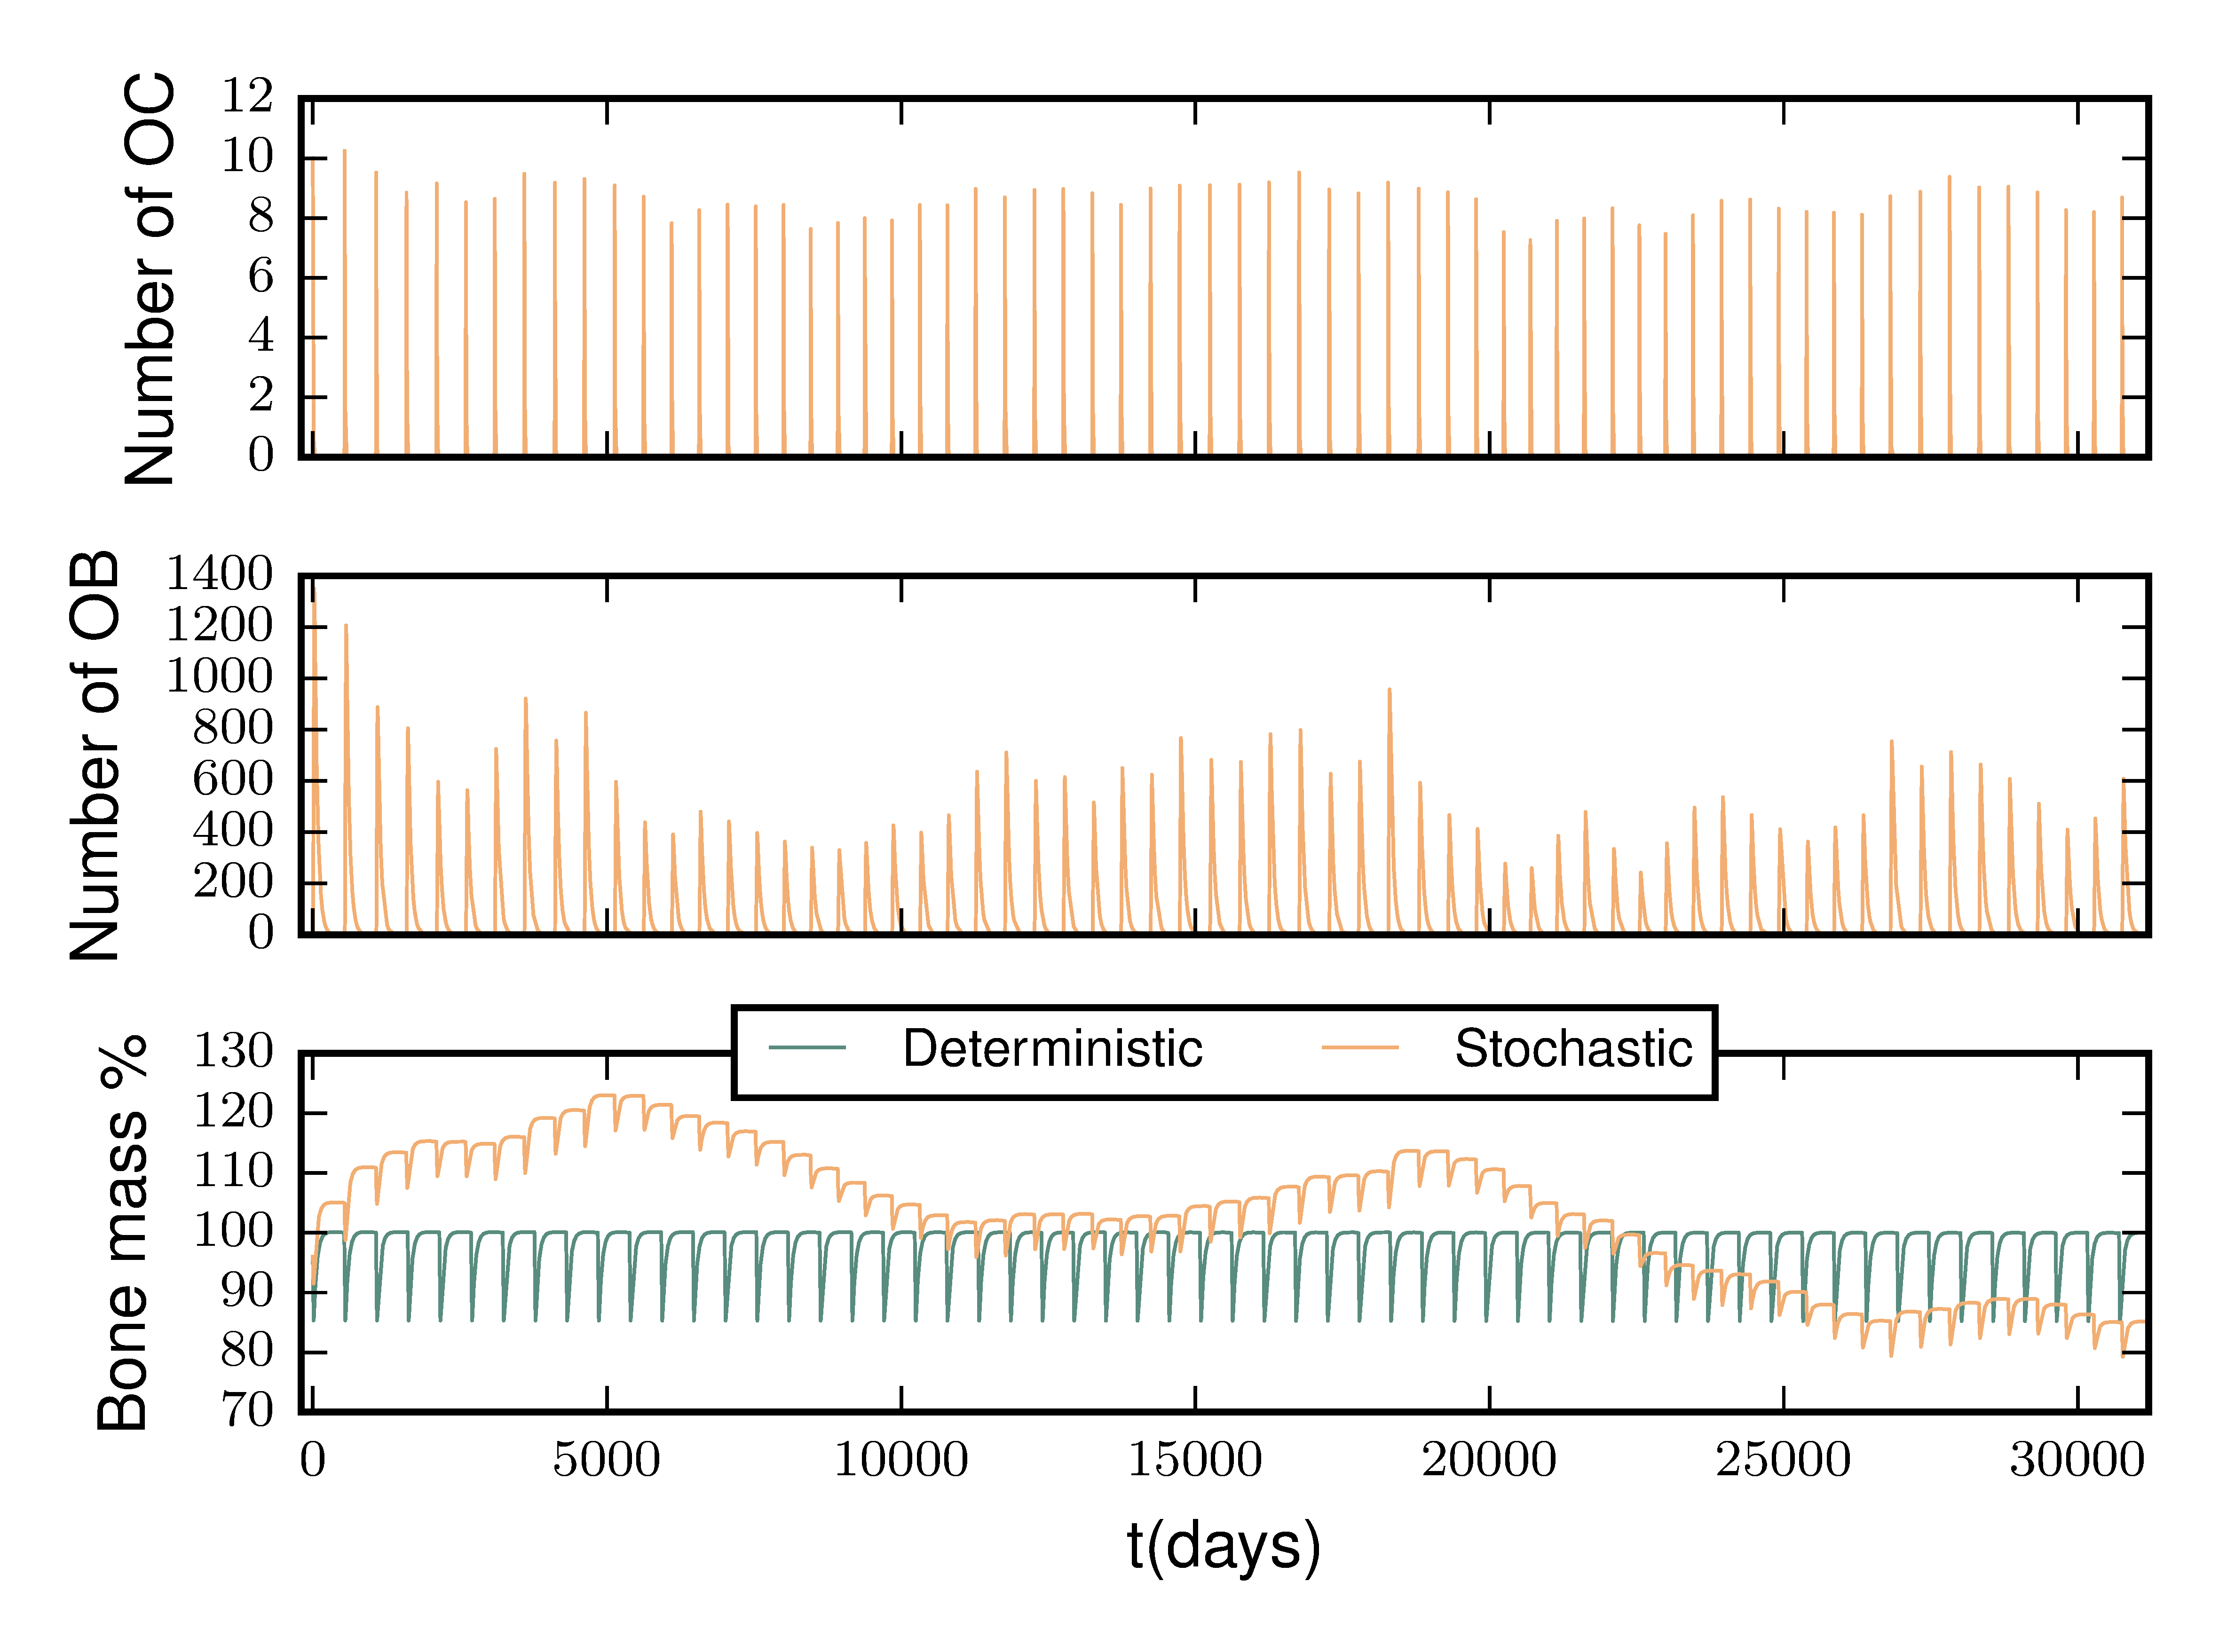
\includegraphics[width=\textwidth,keepaspectratio]{%
		./IMAGES/LongShortTime/longPahtBoneMass.png}
\end{frame}
%%%%%%%%%%%%%%%%%%%%%%%%%%%%%%%%%%%%%%%%%%%%%%%%%%%%%%%%%%%%%%%
\begin{frame}[plain]{Momentos a tiempo corto (13 años)}
	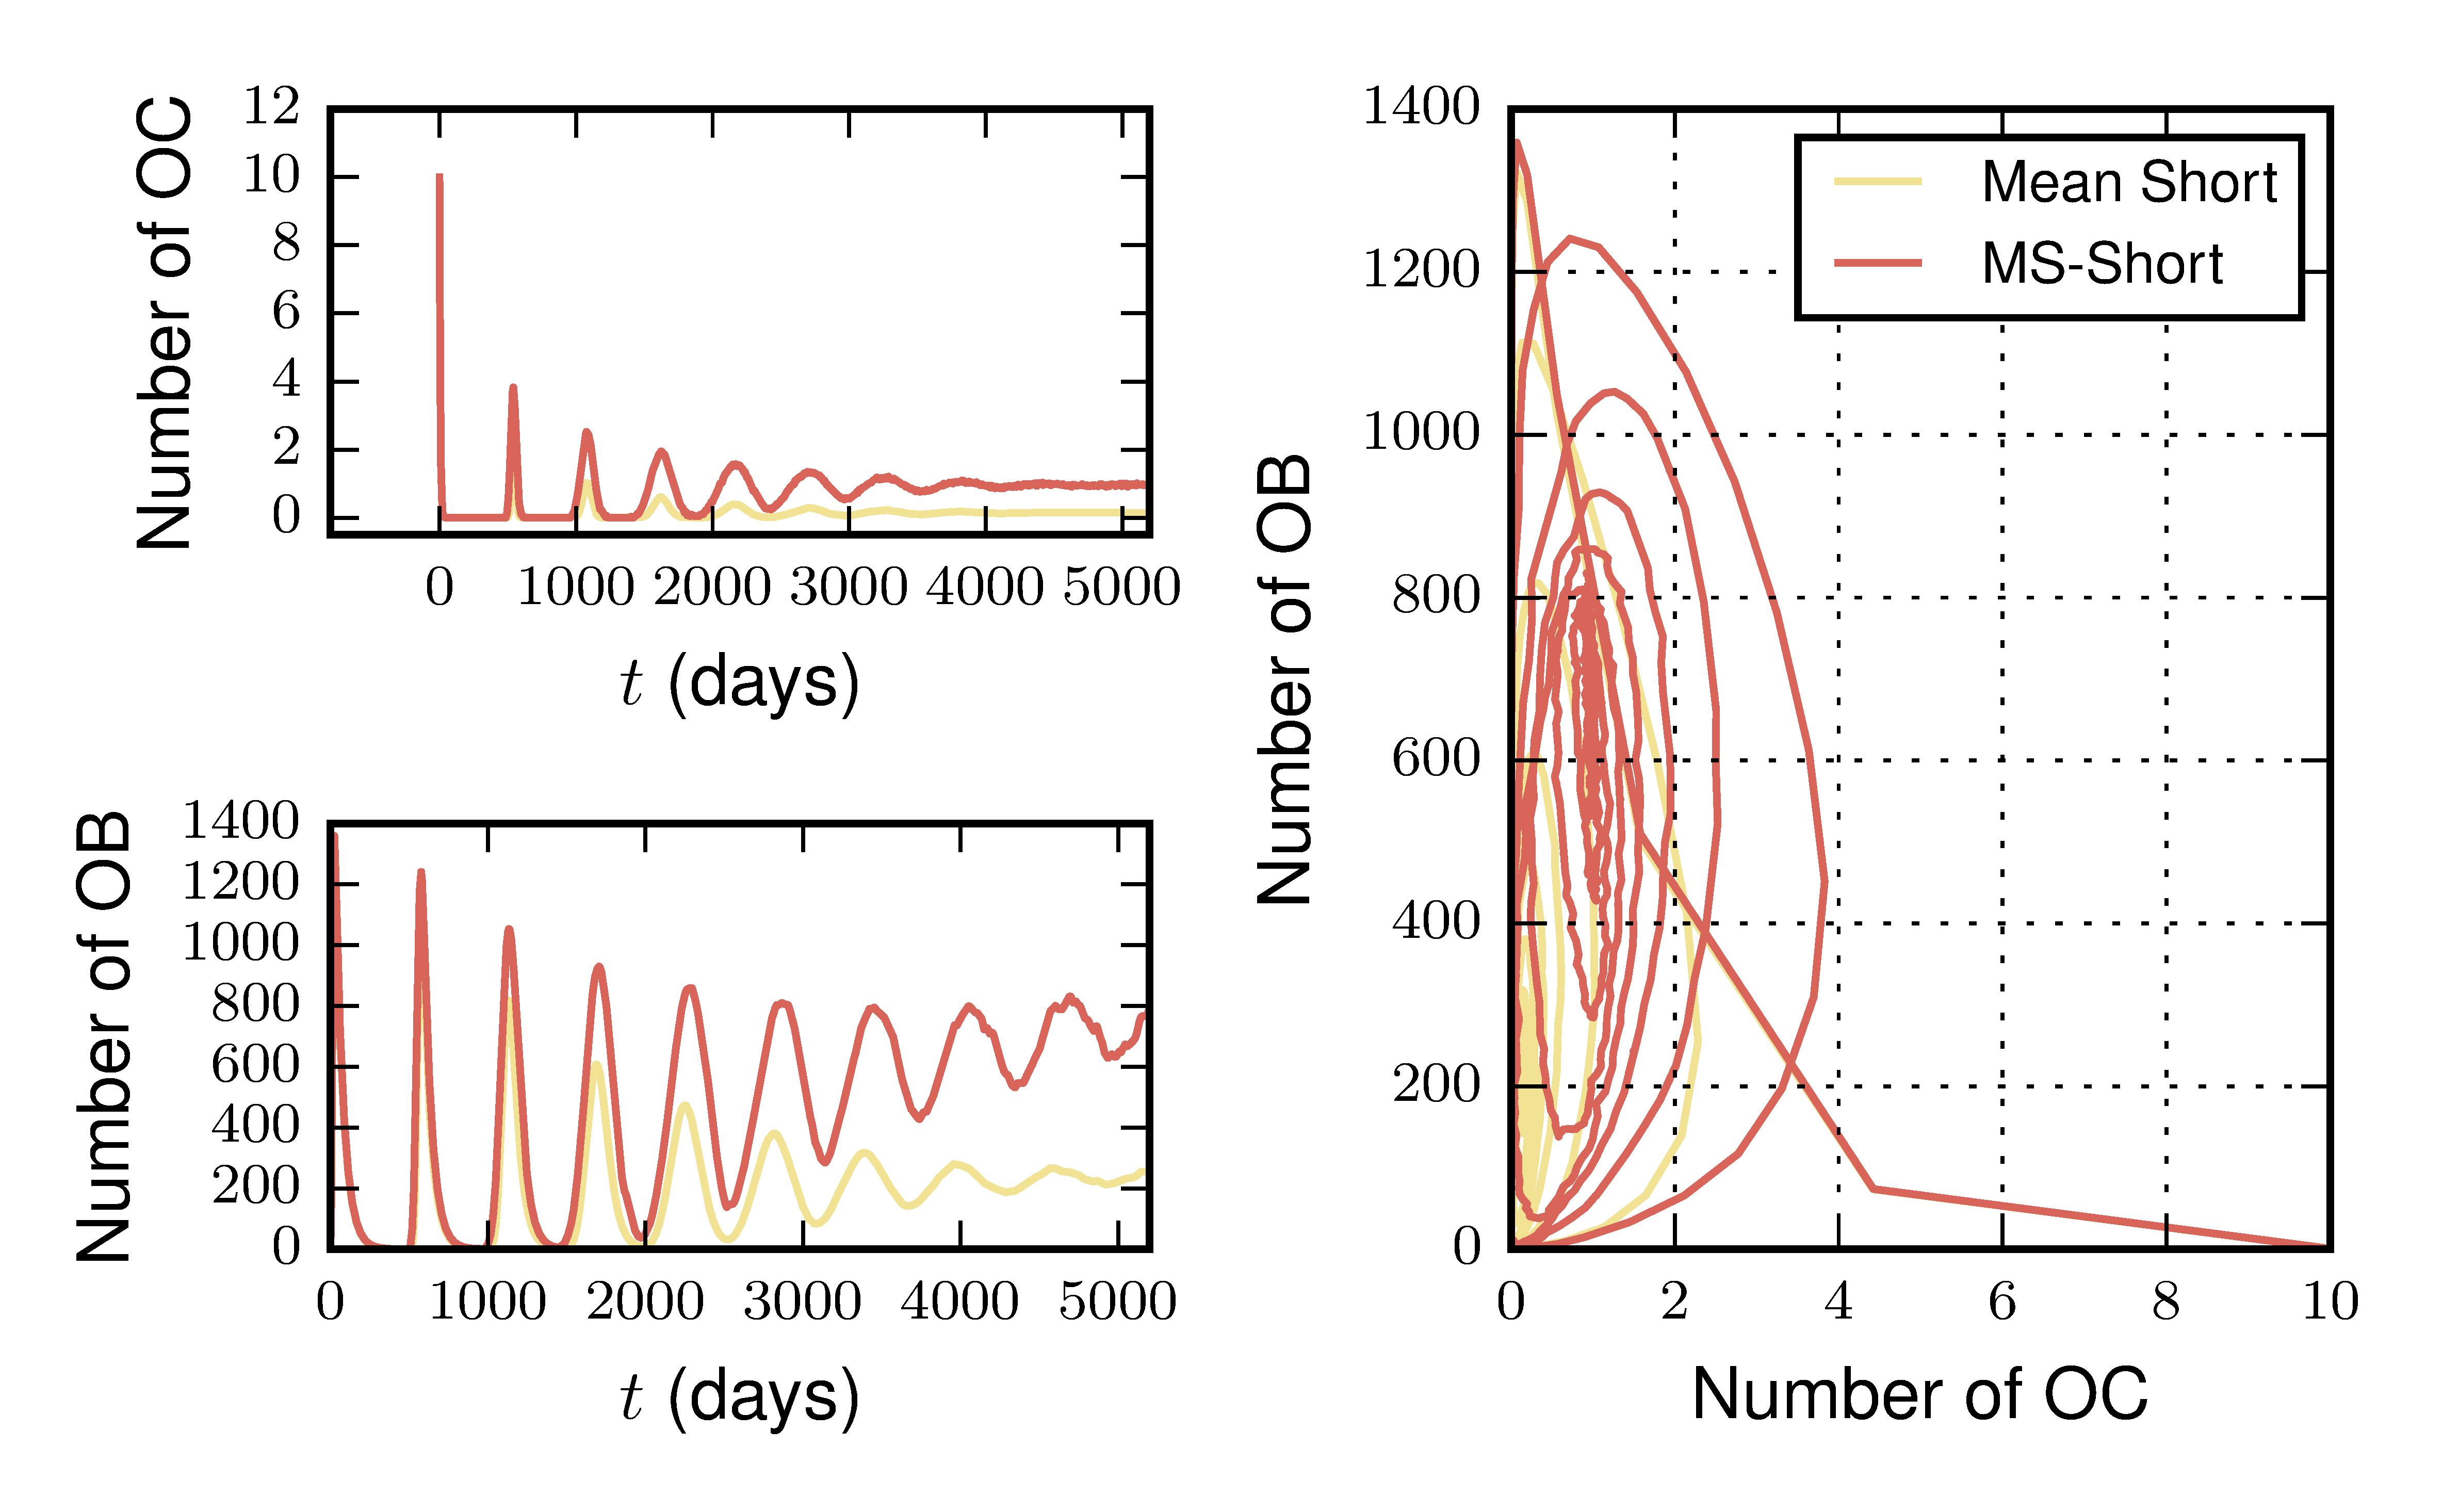
\includegraphics[width=\textwidth,keepaspectratio]{%
		./IMAGES/LongShortTime/shortTimeMoments.png}
\end{frame}
%%%%%%%%%%%%%%%%%%%%%%%%%%%%%%%%%%%%%%%%%%%%%%%%%%%%%%%%%%%%%%%
\begin{frame}[plain]{Momentos a tiempo largo}
	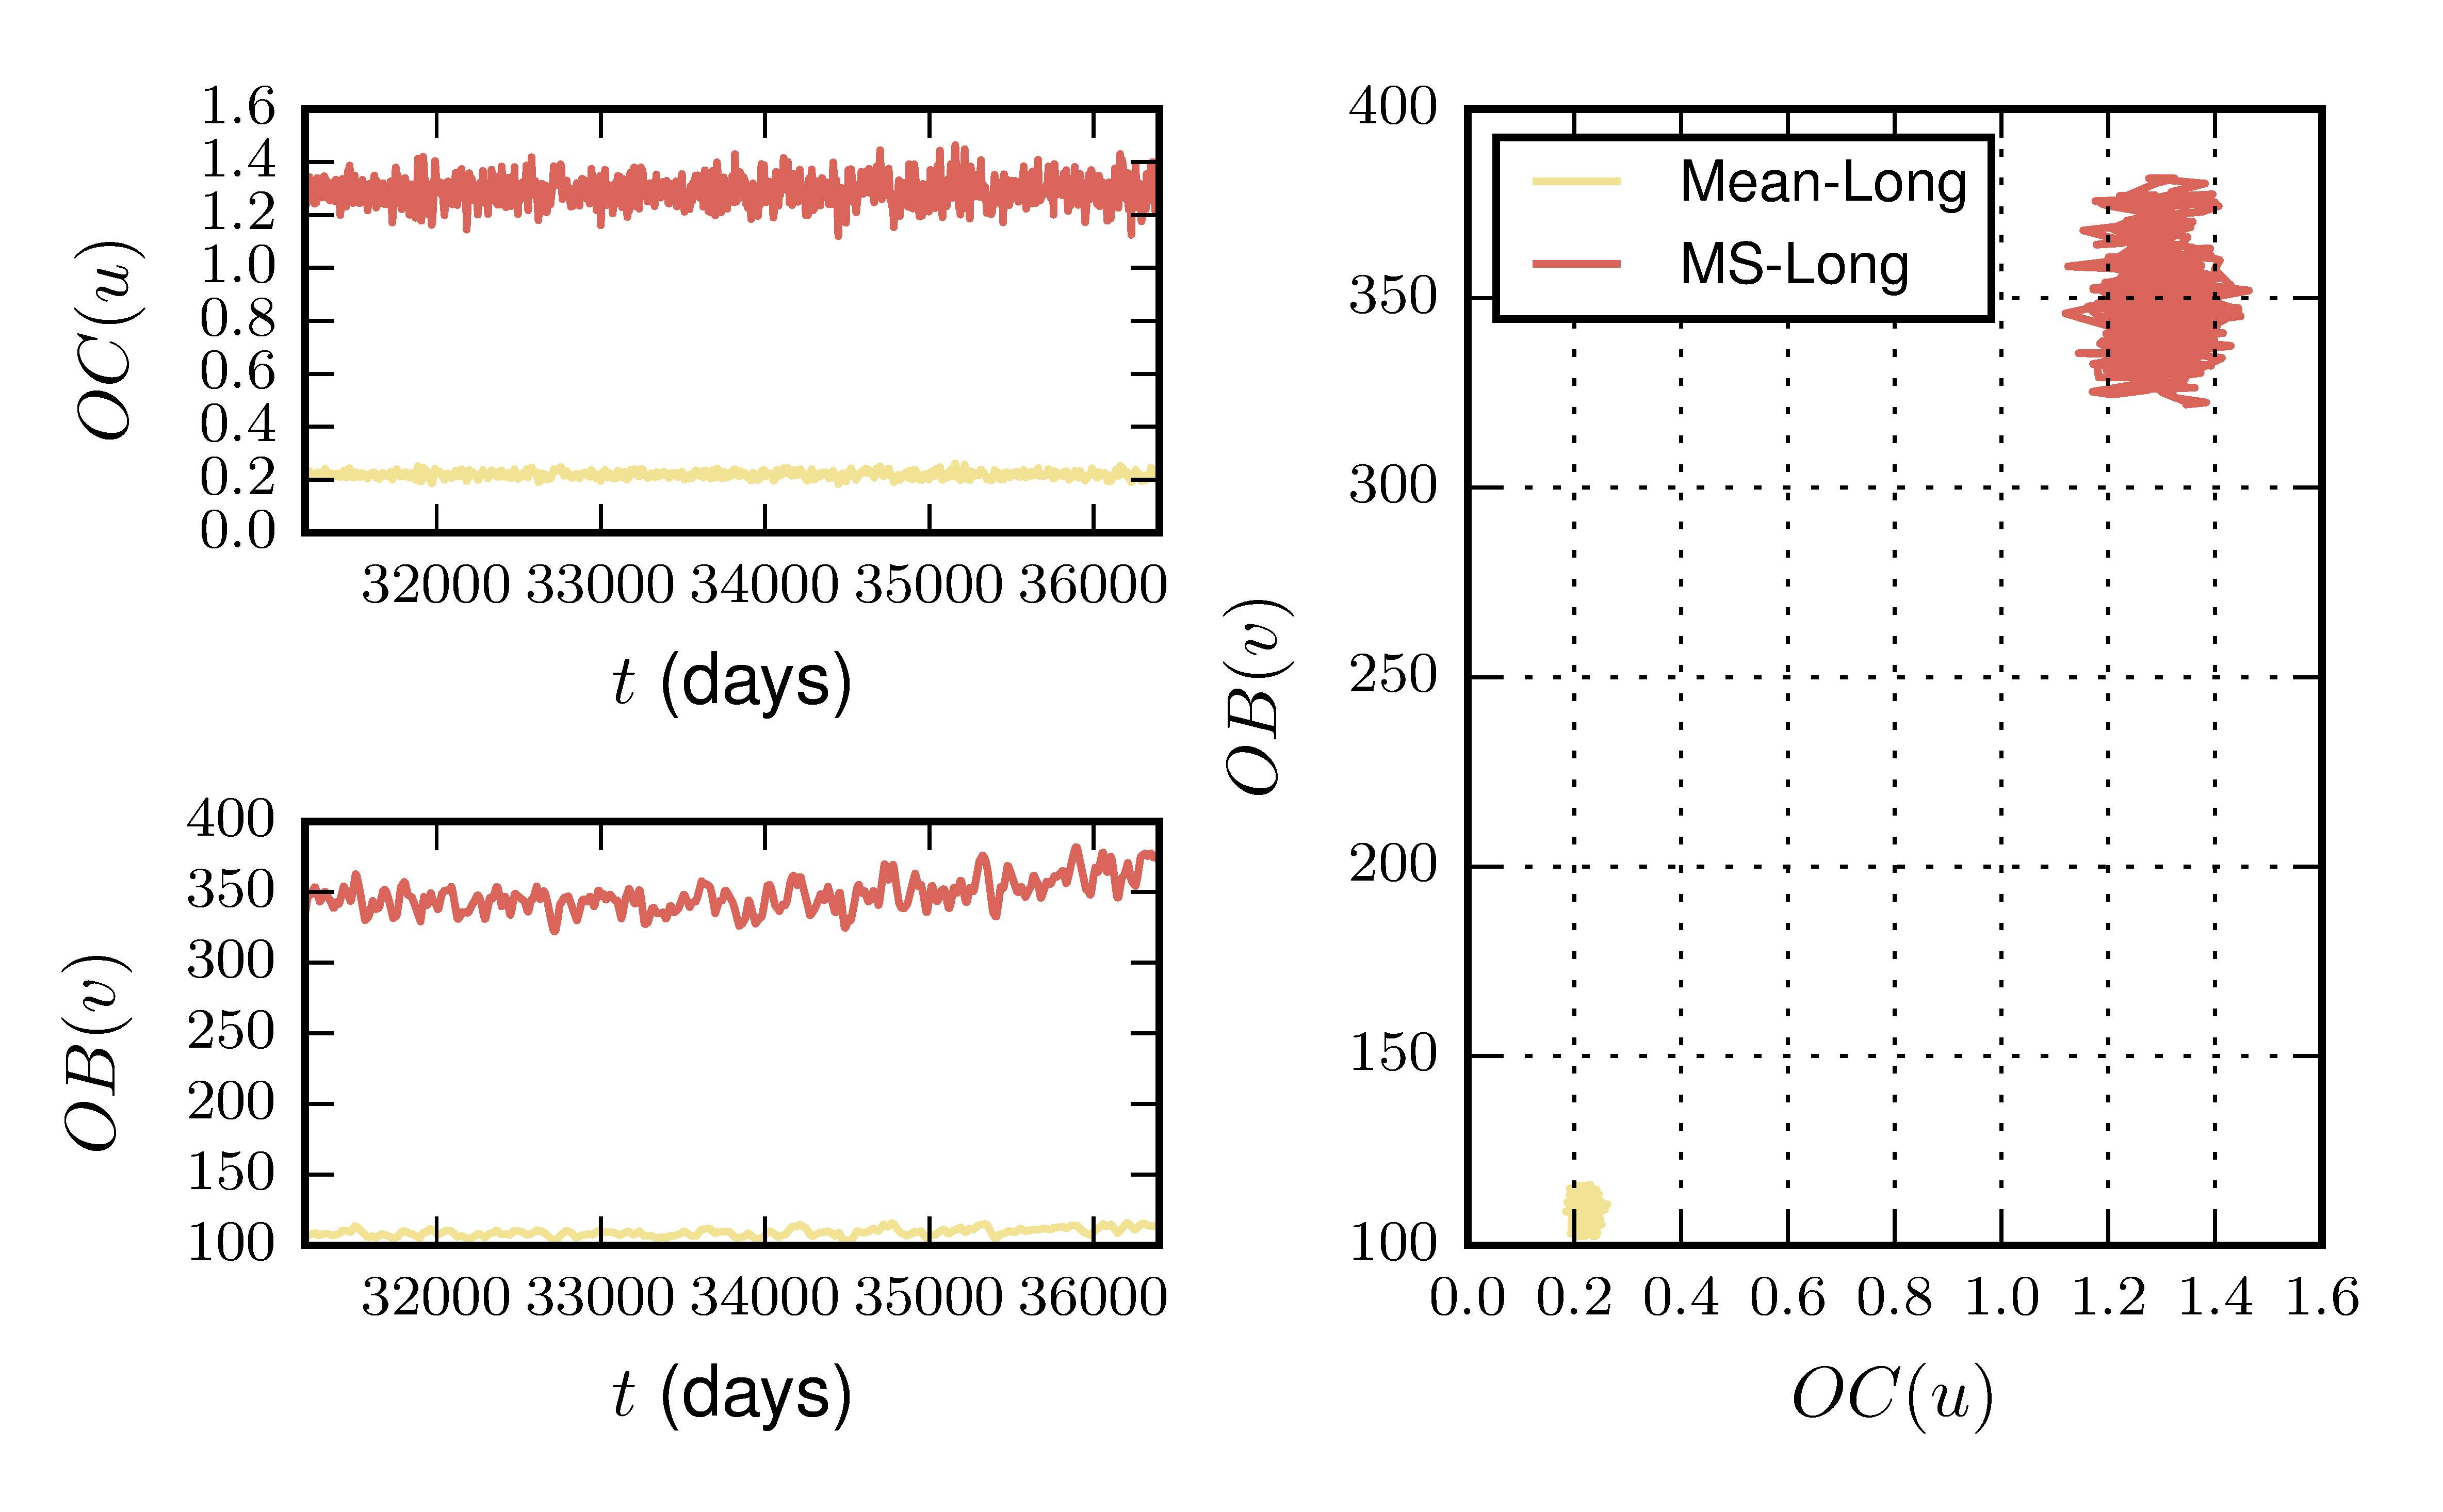
\includegraphics[width=\textwidth,keepaspectratio]{%
		./IMAGES/LongShortTime/longTimeMoments.png}
\end{frame}
%%%%%%%%%%%%%%%%%%%%%%%%%%%%%%%%%%%%%%%%%%%%%%%%%%%%%%%%%%%%%%%

 	\section{Comentarios Finales}
		\begin{frame}[plain]
	\only<1-3>{
	\begin{textblock*}{100mm}(10mm, 40mm)
			\begin{block}{Sometido}    
					\begin{bibunit}[alpha]
					\nocite{Jerez2017}
				%\biblio{CharlaBib.bib}
				\putbib
			\end{bibunit}
			\end{block}   
	\end{textblock*}
	}
 	\only<2>{
		\begin{textblock*}{60mm}(40mm, 20mm)
			\Huge Gracias!!!
		\end{textblock*}
 	}
\end{frame}
\end{document}
